\documentclass[titlepage]{article}
\usepackage[utf8]{inputenc}
\usepackage{amsmath, amssymb, amsthm}
\usepackage{algorithmicx}
\usepackage{graphicx}
\usepackage{subcaption}
\usepackage{listings}
\usepackage{color}
\usepackage{mdframed}
\usepackage{float}
\usepackage{booktabs}
\usepackage{mathtools}

\newcommand{\diag}{\operatorname{diag}}

\definecolor{dkgreen}{rgb}{0,0.6,0}
\definecolor{gray}{rgb}{0.5,0.5,0.5}
\definecolor{mauve}{rgb}{0.58,0,0.82}

\lstset{frame=single,
	language=matlab,
	aboveskip=3mm,
	belowskip=3mm,
	showstringspaces=false,
	columns=flexible,
	basicstyle={\small\ttfamily},
	numbers=none,
	numberstyle=\tiny\color{gray},
	keywordstyle=\color{blue},
	commentstyle=\color{dkgreen},
	stringstyle=\color{mauve},
	breaklines=true,
	breakatwhitespace=true,
	tabsize=3
}

\setlength{\parindent}{0pt}

\title{AAE 50700: Principles of Dynamics\\ Problem Set 6 Report}
\author{Dylan Ashby}
\date{\today}

\begin{document}

\maketitle

\section*{(6.1) Attitude Dynamics with Solar Arrays and Reaction Wheels}

Consider a satellite consisting of a rigid bus $B$, two identical rigid solar arrays $A_1$ and $A_2$, and three reaction wheels, in a torque-free environment. The system center of mass $\mathcal{C}$ is fixed in the inertial frame $\mathcal{N}$. A body-fixed frame $\mathcal{B}:\{\hat{\boldsymbol{b}}_1,\hat{\boldsymbol{b}}_2,\hat{\boldsymbol{b}}_3\}$ is attached to the bus at $\mathcal{C}$. The configuration is detailed below. Fig.~\ref{fig:setup} shows a schematic illustration of the spacecraft.\\

\begin{figure}[H]
	\centering
	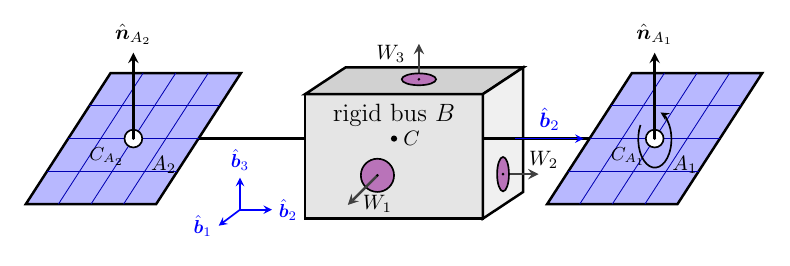
\includegraphics[width=0.8\textwidth]{setup.png}
	\caption{Schematic illustration of the spacecraft considered in PS6.}
	\label{fig:setup}
\end{figure}

\textbf{Solar arrays:} The array centers, $C_{A_1}$ and $C_{A_2}$, are fixed relative to the bus at
\begin{equation}
	\boldsymbol{r}_{C_{A_1}/C}=d\hat{\boldsymbol{b}}_2,\quad\boldsymbol{r}_{C_{A_2}/C}=-d\hat{\boldsymbol{b}}_2.
	\label{eq:rCA}
\end{equation}

Each array rotates about a boom axis parallel to $\hat{\boldsymbol{b}}_2$ and passing through its own center of mass. Since the solar panels need to keep tracking the Sun, both panels have the same normal vector direction:
\begin{equation}
	\hat{\boldsymbol{n}}_{A_1}=\hat{\boldsymbol{n}}_{A_2}=\boldsymbol{R}_2(\beta)\hat{\boldsymbol{b}}_3,
	\label{eq:nA}
\end{equation}
where $\boldsymbol{R}_2(\cdot)$ is a matrix representing a rotation about $\hat{\boldsymbol{b}}_2$. Assume the panel rotation angle $\beta$ is prescribed:
\begin{equation}
	\beta(t)=
	\begin{cases}
		\beta_m\left(10\tau^3-15\tau^4+6\tau^5\right), & 0\leq t\leq t_m,\\
		\beta_m, & t>t_m,
	\end{cases}
	\qquad\tau\coloneqq\frac{t}{t_m}.
	\label{eq:beta}
\end{equation}
where $t_m$, $\beta_m$ are the time and angle at the end of the maneuver, respectively, and $\tau$ is normalized time.\\

Denote by $\boldsymbol{I}_{A0}$ the inertia of each panel about its own center of mass when $\beta=0$. Thus, the panel inertia with the rotation $\beta$ is:
\begin{equation}
	\boldsymbol{I}_A(\beta)=\boldsymbol{R}_2(\beta)\boldsymbol{I}_{A0}\boldsymbol{R}_2^\top(\beta).
	\label{eq:IA}
\end{equation}

\textbf{Reaction wheels (RWs):} Wheel $W_i$ has a fixed spin axis $\hat{\boldsymbol{b}}_i$, axial moment of inertia $J_{w_i}$, and spin angle $\alpha_i$, for $i=1,2,3$. Thus, relevant terms are defined as:
\begin{equation}
	\boldsymbol{\alpha}=[\alpha_1,\alpha_2,\alpha_3]^\top,\qquad\boldsymbol{\Omega}\coloneqq\dot{\boldsymbol{\alpha}},\qquad\boldsymbol{J}_w\coloneqq\diag(J_{w_1},J_{w_2},J_{w_3}).
	\label{eq:rw}
\end{equation}

\textbf{Spacecraft bus:} Denote the bus inertia about $C$ by $\boldsymbol{I}_B$. It includes the inertia of the booms and the wheel transverse inertia components.\\

Express the orientation of $\mathcal{B}$ relative to $\mathcal{N}$ using (3-1-3) Euler angle sequence, defined as $\boldsymbol{\theta}=[\theta_1,\theta_2,\theta_3]^\top$. The relation between the time derivative of $\boldsymbol{\theta}$ and the angular velocity of $\mathcal{B}$ relative to $\mathcal{N}$ is given by:
\begin{equation}
	\boldsymbol{\omega}\coloneqq\prescript{\mathcal{B}}{}{\boldsymbol{\omega}}_{B/N}=\boldsymbol{E}(\boldsymbol{\theta})\dot{\boldsymbol{\theta}},\quad\boldsymbol{E}(\boldsymbol{\theta})=
	\begin{bmatrix}
		\sin\theta_3\sin\theta_2 & \cos\theta_3 & 0 \\
		\sin\theta_2\cos\theta_3 & -\sin\theta_3 & 0 \\
		\cos\theta_2 & 0 & 1
	\end{bmatrix}.
	\label{eq:E}
\end{equation}

\textbf{Generalized coordinates:} Express the generalized coordinates in terms of the bus orientation and wheel spin angles:
\begin{equation}
	\boldsymbol{q}=[\boldsymbol{\theta}^\top,\boldsymbol{\alpha}^\top]^\top.
	\label{eq:gencoord}
\end{equation}

\subsection*{(a): Given}

The above problem formulation.

\subsubsection*{(a.1): Find}

Discuss why it makes sense to not include $\beta(t)$ in the generalized coordinates Eq.~(\ref{eq:gencoord}).\\

\textbf{Analysis/Conclusions:}\\

\begin{mdframed}[linewidth=1pt, innertopmargin=10pt, innerbottommargin=10pt]
	We do not include $\beta$ in the generalized coordinates because its motion is prescribed by Eq.~(\ref{eq:beta}). Generalized coordinates represent the degrees of freedom of the system, and since $\beta(t)$ is known for all time, it is not a free variable and not a degree of freedom. Including it would only add an equation for the drive torque required to control the panels, which is not what we want to find here. Instead, $\beta(t)$ and $\dot{\beta}(t)$ enter the Lagrangian as known functions of time through $\boldsymbol{I}_A(\beta)$ in Eq.~(\ref{eq:IA}) and the angular velocity of the arrays.
\end{mdframed}

\subsubsection*{(a.2): Find}

Let us derive kinetic energy for each component, i.e., bus, solar array assembly, and RW assembly. Denoting them by $T_B$, $T_A$, and $T_W$, respectively, \textbf{show} that they are given by:
\begin{equation}
	\begin{split}
		T_B&=\frac{1}{2}\boldsymbol{\omega}^\top\boldsymbol{I}_B\boldsymbol{\omega},\quad T_A=\frac{1}{2}\left(\boldsymbol{\omega}+\dot{\beta}\hat{\boldsymbol{b}}_2\right)^\top\boldsymbol{I}_{A/C}(\beta)\left(\boldsymbol{\omega}+\dot{\beta}\hat{\boldsymbol{b}}_2\right), \\
		T_W&=\frac{1}{2}\left(\boldsymbol{\omega}+\boldsymbol{\Omega}\right)^\top\boldsymbol{J}_w\left(\boldsymbol{\omega}+\boldsymbol{\Omega}\right)
	\end{split}
	\label{eq:T}
\end{equation}
where $\boldsymbol{I}_{A/C}(\beta)$ is the combined array inertia about $C$, given by:
\begin{equation}
	\boldsymbol{I}_{A/C}(\beta)=2\boldsymbol{I}_A(\beta)+2m_Ad^2\left(I_3-\hat{\boldsymbol{b}}_2\hat{\boldsymbol{b}}_2^\top\right)
	\label{eq:IAC}
\end{equation}

\textbf{Analysis/Conclusions:}\\

It is known that the kinetic energy of a rotating body is half the moment of inertia $I$ times the angular velocity $\omega$ squared. This is generalized to three dimensions by using the moment of inertia tensor $\boldsymbol{I}$ and taking the inner product of the angular velocity vector $\boldsymbol{\omega}$:
\begin{equation}
	T=\frac{1}{2}I\omega^2,\quad T=\frac{1}{2}\boldsymbol{\omega}^\top\boldsymbol{I}\boldsymbol{\omega}
\end{equation}

\begin{mdframed}[linewidth=1pt, innertopmargin=10pt, innerbottommargin=10pt]
	For the equation of the kinetic energy of the bus $T_B$, we can substitute in the inertia tensor of the bus $\boldsymbol{I}_B$ and the angular velocity of the bus $\boldsymbol{\omega}$ (which happens to use the same symbol in this case). Since $\boldsymbol{\theta}$ measures the orientation of the $\mathcal{B}$-frame with respect to the $\mathcal{N}$-frame, the inertial angular velocity of the bus follows directly from Eq.~(\ref{eq:E}), $\boldsymbol{\omega}=\boldsymbol{E}(\boldsymbol{\theta})\dot{\boldsymbol{\theta}}$, and depends only on the generalized coordinates $\boldsymbol{\theta}$ and their rates $\dot{\boldsymbol{\theta}}$. Thus, the kinetic energy of the bus is:
	\begin{equation}
		T_B=\frac{1}{2}\dot{\boldsymbol{\theta}}^\top\boldsymbol{E}^\top(\boldsymbol{\theta})\boldsymbol{I}_B\boldsymbol{E}(\boldsymbol{\theta})\dot{\boldsymbol{\theta}}=\frac{1}{2}\boldsymbol{\omega}^\top\boldsymbol{I}_B\boldsymbol{\omega}
		\label{eq:TB}
	\end{equation}
\end{mdframed}

\begin{mdframed}[linewidth=1pt, innertopmargin=10pt, innerbottommargin=10pt]
	The kinetic energy of the reaction wheels $T_W$ follows a similar structure to the bus kinetic energy, but with an additional degree of rotation with respect to the $\mathcal{N}$-frame, modeled by the angles of rotation $\boldsymbol{\alpha}$, where each angle is the rotation of one of the three wheels relative to the bus. Since each wheel's spin is aligned with one of the $\mathcal{B}$-frame axes, its spin rate $\dot{\alpha}_i=\Omega_i$ simply adds to the bus angular velocity component $\omega_i$ along that same axis. So we can represent the angular rates of the reaction wheels as:
	\begin{equation}
		\boldsymbol{\omega}+\dot{\boldsymbol{\alpha}}=\boldsymbol{\omega}+\boldsymbol{\Omega}
	\end{equation}
	Only the wheels' axial inertias $\boldsymbol{J}_w$ are needed here, as their transverse inertia components are already included in $\boldsymbol{I}_B$. Thus, we can substitute in $\boldsymbol{J}_w$ for the inertia tensor, and the kinetic energy of the reaction wheels is:
	\begin{equation}
		T_W=\frac{1}{2}(\boldsymbol{\omega}+\boldsymbol{\Omega})^\top\boldsymbol{J}_w(\boldsymbol{\omega}+\boldsymbol{\Omega})
	\end{equation}
\end{mdframed}

The arrays' kinetic energy follows a similar structure for the angular rate component, with some additional steps for the inertia tensor.\\

First, we know the solar arrays are, like the reaction wheels, mounted to the bus with their rotational axes aligned with a single axis of the body frame. The orientation of the solar panels is given in Eq.~(\ref{eq:nA}) as the vector normal to the surface of the two panels. Specifically, both panels are always oriented in the same direction and rotate together by angle $\beta$ about $\hat{\boldsymbol{b}}_2$. An angular rate vector always points in the direction of its axis of rotation, with magnitude equal to the rate of change of the rotation angle, so we can simply represent the angular rate of the solar panels relative to the $\mathcal{B}$-frame as:
\begin{equation}
	\dot{\beta}\hat{\boldsymbol{b}}_2
\end{equation}

Then the structure follows the same idea as the reaction wheels, where the angular rate of the arrays aligns with the $\hat{\boldsymbol{b}}_2$ axis of the bus and adds directly to the bus angular velocity, giving the angular rate of the solar panels relative to the $\mathcal{N}$-frame as:
\begin{equation}
	\boldsymbol{\omega}+\dot{\beta}\hat{\boldsymbol{b}}_2
	\label{eq:omegaA}
\end{equation}

Then, the inertia tensor of each array is given by $\boldsymbol{I}_A$. However, there are two arrays who are offset from the center of mass. This means we must derive the offset inertia tensor of the arrays by the parallel axis theorem, then add the two derivations together to get the inertia tensor of the combined two-array system $\boldsymbol{I}_{A/C}$.\\

Recall the parallel axis theorem says we can find inertia tensor displaced from a center of mass $\boldsymbol{I}_P$ by using the following expression where $\boldsymbol{d}$ is a displacement vector, and $\boldsymbol{I}_c$ is the inertia tensor of the object relative to its own center of mass:
\begin{equation}
	\boldsymbol{I}_P=\boldsymbol{I}_c+m(\|\boldsymbol{d}\|^2I_3-\boldsymbol{d}\boldsymbol{d}^\top)
\end{equation}

From the problem definition we know the displacement of the two panels are given in Eq~(\ref{eq:rCA}) as $\boldsymbol{r}_{C_{A_1}/C}$ and $\boldsymbol{r}_{C_{A_2}/C}$. Using $\boldsymbol{I}_A$ as the $\boldsymbol{I}_c$ value, and $m_A$ to represent the mass of an array, we find the offset tensors to be:
\begin{equation}
	\begin{split}
		\boldsymbol{I}_{A1/C}&=\boldsymbol{I}_A+m_A\left(\|\boldsymbol{r}_{C_{A_1}/C}\|^2I_3-\boldsymbol{r}_{C_{A_1}/C}\boldsymbol{r}_{C_{A_1}/C}^\top\right) \\
		&=\boldsymbol{I}_A+m_A\left(\|d\hat{\boldsymbol{b}}_2\|^2I_3-(d\hat{\boldsymbol{b}}_2)(d\hat{\boldsymbol{b}}_2)^\top\right) \\
		&=\boldsymbol{I}_A+m_A\left(d^2I_3-d^2\hat{\boldsymbol{b}}_2\hat{\boldsymbol{b}}_2^\top\right) \\
		&=\boldsymbol{I}_A+m_Ad^2\left(I_3-\hat{\boldsymbol{b}}_2\hat{\boldsymbol{b}}_2^\top\right)
	\end{split}
\end{equation}

And the negative sign cancels with $\boldsymbol{r}_{C_{A_2}/C}$:
\begin{equation}
	\begin{split}
		\boldsymbol{I}_{A2/C}&=\boldsymbol{I}_A+m_A\left(\|\boldsymbol{r}_{C_{A_2}/C}\|^2I_3-\boldsymbol{r}_{C_{A_2}/C}\boldsymbol{r}_{C_{A_2}/C}^\top\right) \\
		&=\boldsymbol{I}_A+m_A\left(\|-d\hat{\boldsymbol{b}}_2\|^2I_3-(-d\hat{\boldsymbol{b}}_2)(-d\hat{\boldsymbol{b}}_2)^\top\right) \\
		&=\boldsymbol{I}_A+m_A\left(d^2I_3-d^2\hat{\boldsymbol{b}}_2\hat{\boldsymbol{b}}_2^\top\right) \\
		&=\boldsymbol{I}_A+m_Ad^2\left(I_3-\hat{\boldsymbol{b}}_2\hat{\boldsymbol{b}}_2^\top\right)
	\end{split}
\end{equation}

  So, if we add together the two tensors to get $\boldsymbol{I}_{A/C}$ we get:
\begin{equation}
	\begin{split}
		\boldsymbol{I}_{A/C}&=\boldsymbol{I}_{A1/C}+\boldsymbol{I}_{A2/C} \\
		&=\left(\boldsymbol{I}_A+m_Ad^2\left(I_3-\hat{\boldsymbol{b}}_2\hat{\boldsymbol{b}}_2^\top\right)\right)+\left(\boldsymbol{I}_A+m_Ad^2\left(I_3-\hat{\boldsymbol{b}}_2\hat{\boldsymbol{b}}_2^\top\right)\right) \\
		&=2\boldsymbol{I}_A+2m_Ad^2\left(I_3-\hat{\boldsymbol{b}}_2\hat{\boldsymbol{b}}_2^\top\right)
	\end{split}
	\label{eq:IACsum}
\end{equation}

\begin{mdframed}[linewidth=1pt, innertopmargin=10pt, innerbottommargin=10pt]
	Thus, with the angular rate found in Eq.~(\ref{eq:omegaA}) and the combined inertia tensor found in Eq.~(\ref{eq:IACsum}), we define the kinetic energy $T_A$ as:
	\begin{equation}
		\begin{split}
			T_A&=\frac{1}{2}\left(\boldsymbol{\omega}+\dot{\beta}\hat{\boldsymbol{b}}_2\right)^\top\boldsymbol{I}_{A/C}\left(\boldsymbol{\omega}+\dot{\beta}\hat{\boldsymbol{b}}_2\right) \\
			&=\frac{1}{2}\left(\boldsymbol{\omega}+\dot{\beta}\hat{\boldsymbol{b}}_2\right)^\top\left(2\boldsymbol{I}_A+2m_Ad^2\left(I_3-\hat{\boldsymbol{b}}_2\hat{\boldsymbol{b}}_2^\top\right)\right)\left(\boldsymbol{\omega}+\dot{\beta}\hat{\boldsymbol{b}}_2\right)
		\end{split}
	\end{equation}
\end{mdframed}

\subsubsection*{(a.3): Find}

Noting that the total kinetic energy is $T=T_B+T_A+T_W$, derive the Lagrangian $L$ for this system and express it in a form that explicitly depends on $(\boldsymbol{q},\dot{\boldsymbol{q}})$ by eliminating $\boldsymbol{\omega}$, $\boldsymbol{\Omega}$ from $L$.\\

\textbf{Analysis/Conclusions:}\\

In this model, there is no potential energy $V$ present, so the Lagrangian $L$ is equivalent to the total kinetic energy $T$. So, we can begin to write the Lagrangian as:
\begin{equation}
	\begin{split}
		L&=T_B+T_A+T_W \\
		&=\frac{1}{2}\boldsymbol{\omega}^\top\boldsymbol{I}_B\boldsymbol{\omega}+\frac{1}{2}\left(\boldsymbol{\omega}+\dot{\beta}\hat{\boldsymbol{b}}_2\right)^\top\boldsymbol{I}_{A/C}(\beta)\left(\boldsymbol{\omega}+\dot{\beta}\hat{\boldsymbol{b}}_2\right)+\frac{1}{2}\left(\boldsymbol{\omega}+\boldsymbol{\Omega}\right)^\top\boldsymbol{J}_w\left(\boldsymbol{\omega}+\boldsymbol{\Omega}\right) \\
		&=\frac{1}{2}\left(\boldsymbol{\omega}^\top\boldsymbol{I}_B\boldsymbol{\omega}+\left(\boldsymbol{\omega}+\dot{\beta}\hat{\boldsymbol{b}}_2\right)^\top\boldsymbol{I}_{A/C}(\beta)\left(\boldsymbol{\omega}+\dot{\beta}\hat{\boldsymbol{b}}_2\right)+\left(\boldsymbol{\omega}+\boldsymbol{\Omega}\right)^\top\boldsymbol{J}_w\left(\boldsymbol{\omega}+\boldsymbol{\Omega}\right)\right)
	\end{split}
\end{equation}

Then to put it in the form that depends on $(\boldsymbol{q},\dot{\boldsymbol{q}})$, the problem definition explicitly defines $\boldsymbol{\Omega}$ as equivalent to $\dot{\boldsymbol{\alpha}}$ and also relates $\boldsymbol{\omega}$ to $\boldsymbol{\theta}$ by:
\begin{equation}
	\boldsymbol{\omega}=\boldsymbol{E}(\boldsymbol{\theta})\dot{\boldsymbol{\theta}},\quad\text{Where:}\quad\boldsymbol{E}(\boldsymbol{\theta})=
	\begin{bmatrix}
		\sin\theta_3\sin\theta_2 & \cos\theta_3 & 0 \\
		\sin\theta_2\cos\theta_3 & -\sin\theta_3 & 0 \\
		\cos\theta_2 & 0 & 1
	\end{bmatrix}
\end{equation}

\begin{mdframed}[linewidth=1pt, innertopmargin=10pt, innerbottommargin=10pt]
	So these substitute into the Lagrangian as:
	\begin{equation}
		\begin{split}
			L&=\frac{1}{2}\bigg(\left(\boldsymbol{E}(\boldsymbol{\theta})\dot{\boldsymbol{\theta}}\right)^\top\boldsymbol{I}_B\left(\boldsymbol{E}(\boldsymbol{\theta})\dot{\boldsymbol{\theta}}\right) \\
			&\quad+\left(\boldsymbol{E}(\boldsymbol{\theta})\dot{\boldsymbol{\theta}}+\dot{\beta}\hat{\boldsymbol{b}}_2\right)^\top\boldsymbol{I}_{A/C}(\beta)\left(\boldsymbol{E}(\boldsymbol{\theta})\dot{\boldsymbol{\theta}}+\dot{\beta}\hat{\boldsymbol{b}}_2\right) \\
			&\quad+\left(\boldsymbol{E}(\boldsymbol{\theta})\dot{\boldsymbol{\theta}}+\dot{\boldsymbol{\alpha}}\right)^\top\boldsymbol{J}_w\left(\boldsymbol{E}(\boldsymbol{\theta})\dot{\boldsymbol{\theta}}+\dot{\boldsymbol{\alpha}}\right)\bigg) \\
			\\
			&\text{Where:}\quad\boldsymbol{E}(\boldsymbol{\theta})=
			\begin{bmatrix}
				\sin\theta_3\sin\theta_2 & \cos\theta_3 & 0 \\
				\sin\theta_2\cos\theta_3 & -\sin\theta_3 & 0 \\
				\cos\theta_2 & 0 & 1
			\end{bmatrix}
		\end{split}
		\label{eq:lagrangian}
	\end{equation}
	Which gives the Lagrangian in a form that explicitly depends on $(\boldsymbol{q},\dot{\boldsymbol{q}})$.
\end{mdframed}

\subsubsection*{(a.4): Find}

Let $u_i$ be the motor torque applied to $W_i$, and $\boldsymbol{u}=[u_1,u_2,u_3]^\top$. Derive the EOM using Lagrange's equations, and show the result in a vector-matrix form: $\boldsymbol{M}(\boldsymbol{q},t)\ddot{\boldsymbol{q}}=f(\boldsymbol{q},\dot{\boldsymbol{q}},t,\boldsymbol{u})$.\\

\textbf{Analysis/Conclusions:}\\

Before we can derive the Lagrange equations, we must first determine the generalized non-conservative forces, which in this scenario come only from the motor torques $\boldsymbol{u}$. We relate $\boldsymbol{u}$ to $\boldsymbol{q}$ through virtual work. If we consider virtual work from the perspective of a torque times an angle, we know the torques themselves act directly on the angles $\boldsymbol{\alpha}$ since the torques are acting directly on the reaction wheels. This means that:
\begin{equation}
	\begin{split}
		\delta W&=\boldsymbol{u}^\top\delta\boldsymbol{\alpha} \\
		&=\left(u_1\hat{\boldsymbol{b}}_1+u_2\hat{\boldsymbol{b}}_2+u_3\hat{\boldsymbol{b}}_3\right)^\top\left(\delta\alpha_1\hat{\boldsymbol{b}}_1+\delta\alpha_2\hat{\boldsymbol{b}}_2+\delta\alpha_3\hat{\boldsymbol{b}}_3\right) \\
		&= u_1\delta\alpha_1+u_2\delta\alpha_2+u_3\delta\alpha_3 \\
		&=Q_{\alpha_1}\delta\alpha_1 + Q_{\alpha_2}\delta\alpha_2 + Q_{\alpha_3}\delta\alpha_3=\boldsymbol{Q}_\alpha^\top\delta\boldsymbol{\alpha}\\
		\\
		&\text{So: }Q_{\alpha_1}=u_1,\quad Q_{\alpha_2}=u_2,\quad Q_{\alpha_3}=u_3
	\end{split}
\end{equation}
Where $Q_{\alpha_i}$ is the generalized non-conservative force associated with each of the three $\alpha$ angles. This relates each torque directly to its own wheel angle and leaves no remaining non-conservative forces, so the non-conservative forces related to $\theta$ angles are all equal to zero.
\begin{equation}
	Q_{\theta_1}=0,\quad Q_{\theta_2}=0,\quad Q_{\theta_3}=0
\end{equation}

Then, we define the following quantities to make the EoM derivation via Lagrange's equation with the Lagrangian in Eq.~(\ref{eq:lagrangian}) simpler.\\

First we define total spacecraft angular momentum about the CoM $\mathcal{C}$ as:
\begin{equation}
	\boldsymbol{H}_S=\boldsymbol{I}_B\boldsymbol{\omega}+\boldsymbol{I}_{A/C}\left(\boldsymbol{\omega}+\dot{\beta}\hat{\boldsymbol{b}}_2\right)+\boldsymbol{J}_w\left(\boldsymbol{\omega}+\boldsymbol{\Omega}\right)
\end{equation}

Then we define instantaneous total spacecraft inertia about $\mathcal{C}$ as:
\begin{equation}
	\boldsymbol{I}_S=\boldsymbol{I}_B+\boldsymbol{I}_{A/C}+\boldsymbol{J}_w
\end{equation}

So, we then apply Lagrange's equation to each coordinate $q_i$ in $\boldsymbol{q}$, which we group into the $\boldsymbol{\theta}$ and $\boldsymbol{\alpha}$ blocks:
\begin{equation}
	\frac{d}{dt}\left(\frac{\partial L}{\partial\dot{q}_i}\right)-\frac{\partial L}{\partial q_i}=Q_i,\qquad i=1,\dots,6
\end{equation}

Below we solve the partials individually for easier reading. Because of the usage of $\boldsymbol{\theta}$ and $\boldsymbol{\alpha}$ as vectors in the Lagrangian, the most convenient form ended up being taking the derivatives with respect to $\boldsymbol{\theta}$ and $\boldsymbol{\alpha}$ rather than component-wise:
\begin{equation}
	\begin{split}
		\frac{\partial L}{\partial\boldsymbol{\theta}}&=\frac{1}{2}\bigg(\frac{\partial}{\partial\boldsymbol{\theta}}\left(\boldsymbol{E}(\boldsymbol{\theta})\dot{\boldsymbol{\theta}}\right)^\top\boldsymbol{I}_B\left(\boldsymbol{E}(\boldsymbol{\theta})\dot{\boldsymbol{\theta}}\right) \\
		&\quad+\frac{\partial}{\partial\boldsymbol{\theta}}\left(\boldsymbol{E}(\boldsymbol{\theta})\dot{\boldsymbol{\theta}}+\dot{\beta}\hat{\boldsymbol{b}}_2\right)^\top\boldsymbol{I}_{A/C}(\beta)\left(\boldsymbol{E}(\boldsymbol{\theta})\dot{\boldsymbol{\theta}}+\dot{\beta}\hat{\boldsymbol{b}}_2\right) \\
		&\quad+\frac{\partial}{\partial\boldsymbol{\theta}}\left(\boldsymbol{E}(\boldsymbol{\theta})\dot{\boldsymbol{\theta}}+\dot{\boldsymbol{\alpha}}\right)^\top\boldsymbol{J}_w\left(\boldsymbol{E}(\boldsymbol{\theta})\dot{\boldsymbol{\theta}}+\dot{\boldsymbol{\alpha}}\right)\bigg)
	\end{split}
	\label{eq:thetaterm}
\end{equation}

Then work out the derivative of each term:
\begin{equation}
	\begin{split}
		&=\frac{\partial}{\partial\boldsymbol{\theta}}\left(\left(\boldsymbol{E}(\boldsymbol{\theta})\dot{\boldsymbol{\theta}}\right)^\top\boldsymbol{I}_B\left(\boldsymbol{E}(\boldsymbol{\theta})\dot{\boldsymbol{\theta}}\right)\right) \\
		&=\left(\frac{\partial\boldsymbol{E}(\boldsymbol{\theta})}{\partial\boldsymbol{\theta}}\dot{\boldsymbol{\theta}}\right)^\top\boldsymbol{I}_B\left(\boldsymbol{E}(\boldsymbol{\theta})\dot{\boldsymbol{\theta}}\right)+\left(\boldsymbol{E}(\boldsymbol{\theta})\dot{\boldsymbol{\theta}}\right)^\top\boldsymbol{I}_B\left(\frac{\partial\boldsymbol{E}(\boldsymbol{\theta})}{\partial\boldsymbol{\theta}}\dot{\boldsymbol{\theta}}\right) \\
		&=2\left(\frac{\partial\boldsymbol{E}(\boldsymbol{\theta})}{\partial\boldsymbol{\theta}}\dot{\boldsymbol{\theta}}\right)^\top\boldsymbol{I}_B\left(\boldsymbol{E}(\boldsymbol{\theta})\dot{\boldsymbol{\theta}}\right) \\
		&=2\left(\frac{\partial\boldsymbol{E}(\boldsymbol{\theta})}{\partial\boldsymbol{\theta}}\dot{\boldsymbol{\theta}}\right)^\top\boldsymbol{I}_B\boldsymbol{\omega}
	\end{split}
\end{equation}

For the array term:
\begin{equation}
	\begin{split}
		&=\frac{\partial}{\partial\boldsymbol{\theta}}\left(\left(\boldsymbol{E}(\boldsymbol{\theta})\dot{\boldsymbol{\theta}}+\dot{\beta}\hat{\boldsymbol{b}}_2\right)^\top\boldsymbol{I}_{A/C}(\beta)\left(\boldsymbol{E}(\boldsymbol{\theta})\dot{\boldsymbol{\theta}}+\dot{\beta}\hat{\boldsymbol{b}}_2\right)\right) \\
		&=\left(\frac{\partial\boldsymbol{E}(\boldsymbol{\theta})}{\partial\boldsymbol{\theta}}\dot{\boldsymbol{\theta}}\right)^\top\boldsymbol{I}_{A/C}(\beta)\left(\boldsymbol{E}(\boldsymbol{\theta})\dot{\boldsymbol{\theta}}+\dot{\beta}\hat{\boldsymbol{b}}_2\right)+\left(\boldsymbol{E}(\boldsymbol{\theta})\dot{\boldsymbol{\theta}}+\dot{\beta}\hat{\boldsymbol{b}}_2\right)^\top\boldsymbol{I}_{A/C}(\beta)\left(\frac{\partial\boldsymbol{E}(\boldsymbol{\theta})}{\partial\boldsymbol{\theta}}\dot{\boldsymbol{\theta}}\right) \\
		&=2\left(\frac{\partial\boldsymbol{E}(\boldsymbol{\theta})}{\partial\boldsymbol{\theta}}\dot{\boldsymbol{\theta}}\right)^\top\boldsymbol{I}_{A/C}(\beta)\left(\boldsymbol{E}(\boldsymbol{\theta})\dot{\boldsymbol{\theta}}+\dot{\beta}\hat{\boldsymbol{b}}_2\right) \\
		&=2\left(\frac{\partial\boldsymbol{E}(\boldsymbol{\theta})}{\partial\boldsymbol{\theta}}\dot{\boldsymbol{\theta}}\right)^\top\boldsymbol{I}_{A/C}(\beta)\left(\boldsymbol{\omega}+\dot{\beta}\hat{\boldsymbol{b}}_2\right)
	\end{split}
\end{equation}

For the wheel term:
\begin{equation}
	\begin{split}
		&=\frac{\partial}{\partial\boldsymbol{\theta}}\left(\left(\boldsymbol{E}(\boldsymbol{\theta})\dot{\boldsymbol{\theta}}+\dot{\boldsymbol{\alpha}}\right)^\top\boldsymbol{J}_w\left(\boldsymbol{E}(\boldsymbol{\theta})\dot{\boldsymbol{\theta}}+\dot{\boldsymbol{\alpha}}\right)\right) \\
		&=\left(\frac{\partial\boldsymbol{E}(\boldsymbol{\theta})}{\partial\boldsymbol{\theta}}\dot{\boldsymbol{\theta}}\right)^\top\boldsymbol{J}_w\left(\boldsymbol{E}(\boldsymbol{\theta})\dot{\boldsymbol{\theta}}+\dot{\boldsymbol{\alpha}}\right)+\left(\boldsymbol{E}(\boldsymbol{\theta})\dot{\boldsymbol{\theta}}+\dot{\boldsymbol{\alpha}}\right)^\top\boldsymbol{J}_w\left(\frac{\partial\boldsymbol{E}(\boldsymbol{\theta})}{\partial\boldsymbol{\theta}}\dot{\boldsymbol{\theta}}\right) \\
		&=2\left(\frac{\partial\boldsymbol{E}(\boldsymbol{\theta})}{\partial\boldsymbol{\theta}}\dot{\boldsymbol{\theta}}\right)^\top\boldsymbol{J}_w\left(\boldsymbol{E}(\boldsymbol{\theta})\dot{\boldsymbol{\theta}}+\dot{\boldsymbol{\alpha}}\right) \\
		&=2\left(\frac{\partial\boldsymbol{E}(\boldsymbol{\theta})}{\partial\boldsymbol{\theta}}\dot{\boldsymbol{\theta}}\right)^\top\boldsymbol{J}_w\left(\boldsymbol{\omega}+\boldsymbol{\Omega}\right)
	\end{split}
\end{equation}

Note in the above equations, we substitute $\boldsymbol{\omega}$ for $\boldsymbol{E}(\boldsymbol{\theta})\dot{\boldsymbol{\theta}}$ and $\boldsymbol{\Omega}$ for $\dot{\boldsymbol{\alpha}}$ since they have been determined to be equivalent by the problem setup. So, if we substitute these components into Eq.~(\ref{eq:thetaterm}):
\begin{equation}
	\begin{split}
		\frac{\partial L}{\partial\boldsymbol{\theta}}&=\frac{1}{2}\bigg(2\left(\frac{\partial\boldsymbol{E}(\boldsymbol{\theta})}{\partial\boldsymbol{\theta}}\dot{\boldsymbol{\theta}}\right)^\top\boldsymbol{I}_B\boldsymbol{\omega}+2\left(\frac{\partial\boldsymbol{E}(\boldsymbol{\theta})}{\partial\boldsymbol{\theta}}\dot{\boldsymbol{\theta}}\right)^\top\boldsymbol{I}_{A/C}(\beta)\left(\boldsymbol{\omega}+\dot{\beta}\hat{\boldsymbol{b}}_2\right) \\
		&\quad+2\left(\frac{\partial\boldsymbol{E}(\boldsymbol{\theta})}{\partial\boldsymbol{\theta}}\dot{\boldsymbol{\theta}}\right)^\top\boldsymbol{J}_w\left(\boldsymbol{\omega}+\boldsymbol{\Omega}\right)\bigg) \\
		&=\left(\frac{\partial\boldsymbol{E}(\boldsymbol{\theta})}{\partial\boldsymbol{\theta}}\dot{\boldsymbol{\theta}}\right)^\top\left(\boldsymbol{I}_B\boldsymbol{\omega}+\boldsymbol{I}_{A/C}(\beta)\left(\boldsymbol{\omega}+\dot{\beta}\hat{\boldsymbol{b}}_2\right)+\boldsymbol{J}_w\left(\boldsymbol{\omega}+\boldsymbol{\Omega}\right)\right) \\
		&=\left(\frac{\partial\boldsymbol{E}(\boldsymbol{\theta})}{\partial\boldsymbol{\theta}}\dot{\boldsymbol{\theta}}\right)^\top\boldsymbol{H}_S
	\end{split}
\end{equation}
Which makes use of the earlier defined $\boldsymbol{H}_S$ term.\\

Then, we find the partial derivative $\frac{\partial\boldsymbol{E}(\boldsymbol{\theta})}{\partial\boldsymbol{\theta}}$. At this point, it must be done component-wise of $\boldsymbol{\theta}$.\\

For $\theta_1$:
\begin{equation}
	\begin{split}
		\frac{\partial\boldsymbol{E}(\boldsymbol{\theta})}{\partial\theta_1}&=\frac{\partial}{\partial\theta_1}
		\begin{bmatrix}
			\sin\theta_3\sin\theta_2 & \cos\theta_3 & 0 \\
			\sin\theta_2\cos\theta_3 & -\sin\theta_3 & 0 \\
			\cos\theta_2 & 0 & 1
		\end{bmatrix} \\
		&=
		\begin{bmatrix}
			\frac{\partial}{\partial\theta_1}\left(\sin\theta_3\sin\theta_2\right) & \frac{\partial}{\partial\theta_1}\left(\cos\theta_3\right) & \frac{\partial}{\partial\theta_1}\left(0\right) \\
			\frac{\partial}{\partial\theta_1}\left(\sin\theta_2\cos\theta_3\right) & \frac{\partial}{\partial\theta_1}\left(-\sin\theta_3\right) & \frac{\partial}{\partial\theta_1}\left(0\right) \\
			\frac{\partial}{\partial\theta_1}\left(\cos\theta_2\right) & \frac{\partial}{\partial\theta_1}\left(0\right) & \frac{\partial}{\partial\theta_1}\left(1\right)
		\end{bmatrix} \\
		&=
		\begin{bmatrix}
			0 & 0 & 0 \\
			0 & 0 & 0 \\
			0 & 0 & 0 
		\end{bmatrix} \\
	\end{split}
\end{equation}

For $\theta_2$:
\begin{equation}
	\begin{split}
		\frac{\partial\boldsymbol{E}(\boldsymbol{\theta})}{\partial\theta_2}&=\frac{\partial}{\partial\theta_2}
		\begin{bmatrix}
			\sin\theta_3\sin\theta_2 & \cos\theta_3 & 0 \\
			\sin\theta_2\cos\theta_3 & -\sin\theta_3 & 0 \\
			\cos\theta_2 & 0 & 1
		\end{bmatrix} \\
		&=
		\begin{bmatrix}
			\frac{\partial}{\partial\theta_2}\left(\sin\theta_3\sin\theta_2\right) & \frac{\partial}{\partial\theta_2}\left(\cos\theta_3\right) & \frac{\partial}{\partial\theta_2}\left(0\right) \\
			\frac{\partial}{\partial\theta_2}\left(\sin\theta_2\cos\theta_3\right) & \frac{\partial}{\partial\theta_2}\left(-\sin\theta_3\right) & \frac{\partial}{\partial\theta_2}\left(0\right) \\
			\frac{\partial}{\partial\theta_2}\left(\cos\theta_2\right) & \frac{\partial}{\partial\theta_2}\left(0\right) & \frac{\partial}{\partial\theta_2}\left(1\right)
		\end{bmatrix} \\
		&=
		\begin{bmatrix}
			\sin\theta_3\cos\theta_2 & 0 & 0 \\
			\cos\theta_2\cos\theta_3 & 0 & 0 \\
			-\sin\theta_2 & 0 & 0
		\end{bmatrix}
	\end{split}
\end{equation}

For $\theta_3$:
\begin{equation}
	\begin{split}
		\frac{\partial\boldsymbol{E}(\boldsymbol{\theta})}{\partial\theta_3}&=\frac{\partial}{\partial\theta_3}
		\begin{bmatrix}
			\sin\theta_3\sin\theta_2 & \cos\theta_3 & 0 \\
			\sin\theta_2\cos\theta_3 & -\sin\theta_3 & 0 \\
			\cos\theta_2 & 0 & 1
		\end{bmatrix} \\
		&=
		\begin{bmatrix}
			\frac{\partial}{\partial\theta_3}\left(\sin\theta_3\sin\theta_2\right) & \frac{\partial}{\partial\theta_3}\left(\cos\theta_3\right) & \frac{\partial}{\partial\theta_3}\left(0\right) \\
			\frac{\partial}{\partial\theta_3}\left(\sin\theta_2\cos\theta_3\right) & \frac{\partial}{\partial\theta_3}\left(-\sin\theta_3\right) & \frac{\partial}{\partial\theta_3}\left(0\right) \\
			\frac{\partial}{\partial\theta_3}\left(\cos\theta_2\right) & \frac{\partial}{\partial\theta_3}\left(0\right) & \frac{\partial}{\partial\theta_3}\left(1\right)
		\end{bmatrix} \\
		&=
		\begin{bmatrix}
			\cos\theta_3\sin\theta_2 & -\sin\theta_3 & 0 \\
			-\sin\theta_2\sin\theta_3 & -\cos\theta_3 & 0 \\
			0 & 0 & 0
		\end{bmatrix}
	\end{split}
\end{equation}

Then, we find the $\frac{\partial L}{\partial\dot{\boldsymbol{\theta}}}$ evaluation:
\begin{equation}
	\begin{split}
		\frac{\partial L}{\partial\dot{\boldsymbol{\theta}}}&=\frac{1}{2}\bigg(\frac{\partial}{\partial\dot{\boldsymbol{\theta}}}\left(\boldsymbol{E}(\boldsymbol{\theta})\dot{\boldsymbol{\theta}}\right)^\top\boldsymbol{I}_B\left(\boldsymbol{E}(\boldsymbol{\theta})\dot{\boldsymbol{\theta}}\right) \\
		&\quad+\frac{\partial}{\partial\dot{\boldsymbol{\theta}}}\left(\boldsymbol{E}(\boldsymbol{\theta})\dot{\boldsymbol{\theta}}+\dot{\beta}\hat{\boldsymbol{b}}_2\right)^\top\boldsymbol{I}_{A/C}(\beta)\left(\boldsymbol{E}(\boldsymbol{\theta})\dot{\boldsymbol{\theta}}+\dot{\beta}\hat{\boldsymbol{b}}_2\right) \\
		&\quad+\frac{\partial}{\partial\dot{\boldsymbol{\theta}}}\left(\boldsymbol{E}(\boldsymbol{\theta})\dot{\boldsymbol{\theta}}+\dot{\boldsymbol{\alpha}}\right)^\top\boldsymbol{J}_w\left(\boldsymbol{E}(\boldsymbol{\theta})\dot{\boldsymbol{\theta}}+\dot{\boldsymbol{\alpha}}\right)\bigg)
	\end{split}
	\label{eq:thetadotterm}
\end{equation}

Then work out the derivative of each term. This will set up a substitution similar to what was done for $\frac{\partial L}{\partial\boldsymbol{\theta}}$.\\

For the bus term:
\begin{equation}
	\begin{split}
		&=\frac{\partial}{\partial\dot{\boldsymbol{\theta}}}\left(\left(\boldsymbol{E}(\boldsymbol{\theta})\dot{\boldsymbol{\theta}}\right)^\top\boldsymbol{I}_B\left(\boldsymbol{E}(\boldsymbol{\theta})\dot{\boldsymbol{\theta}}\right)\right) \\
		&=\left(\boldsymbol{E}(\boldsymbol{\theta})\frac{\partial\dot{\boldsymbol{\theta}}}{\partial\dot{\boldsymbol{\theta}}}\right)^\top\boldsymbol{I}_B\left(\boldsymbol{E}(\boldsymbol{\theta})\dot{\boldsymbol{\theta}}\right)+\left(\boldsymbol{E}(\boldsymbol{\theta})\dot{\boldsymbol{\theta}}\right)^\top\boldsymbol{I}_B\left(\boldsymbol{E}(\boldsymbol{\theta})\frac{\partial\dot{\boldsymbol{\theta}}}{\partial\dot{\boldsymbol{\theta}}}\right) \\
		&=2\left(\boldsymbol{E}(\boldsymbol{\theta})\frac{\partial\dot{\boldsymbol{\theta}}}{\partial\dot{\boldsymbol{\theta}}}\right)^\top\boldsymbol{I}_B\left(\boldsymbol{E}(\boldsymbol{\theta})\dot{\boldsymbol{\theta}}\right) \\
		&=2\boldsymbol{E}(\boldsymbol{\theta})^\top\boldsymbol{I}_B\boldsymbol{\omega}
	\end{split}
\end{equation}

For the array term:
\begin{equation}
	\begin{split}
		&=\frac{\partial}{\partial\dot{\boldsymbol{\theta}}}\left(\left(\boldsymbol{E}(\boldsymbol{\theta})\dot{\boldsymbol{\theta}}+\dot{\beta}\hat{\boldsymbol{b}}_2\right)^\top\boldsymbol{I}_{A/C}(\beta)\left(\boldsymbol{E}(\boldsymbol{\theta})\dot{\boldsymbol{\theta}}+\dot{\beta}\hat{\boldsymbol{b}}_2\right)\right) \\
		&=\left(\boldsymbol{E}(\boldsymbol{\theta})\frac{\partial\dot{\boldsymbol{\theta}}}{\partial\dot{\boldsymbol{\theta}}}\right)^\top\boldsymbol{I}_{A/C}(\beta)\left(\boldsymbol{E}(\boldsymbol{\theta})\dot{\boldsymbol{\theta}}+\dot{\beta}\hat{\boldsymbol{b}}_2\right)+\left(\boldsymbol{E}(\boldsymbol{\theta})\dot{\boldsymbol{\theta}}+\dot{\beta}\hat{\boldsymbol{b}}_2\right)^\top\boldsymbol{I}_{A/C}(\beta)\left(\boldsymbol{E}(\boldsymbol{\theta})\frac{\partial\dot{\boldsymbol{\theta}}}{\partial\dot{\boldsymbol{\theta}}}\right) \\
		&=2\left(\boldsymbol{E}(\boldsymbol{\theta})\frac{\partial\dot{\boldsymbol{\theta}}}{\partial\dot{\boldsymbol{\theta}}}\right)^\top\boldsymbol{I}_{A/C}(\beta)\left(\boldsymbol{E}(\boldsymbol{\theta})\dot{\boldsymbol{\theta}}+\dot{\beta}\hat{\boldsymbol{b}}_2\right) \\
		&=2\boldsymbol{E}(\boldsymbol{\theta})^\top\boldsymbol{I}_{A/C}(\beta)\left(\boldsymbol{\omega}+\dot{\beta}\hat{\boldsymbol{b}}_2\right)
	\end{split}
\end{equation}

For the wheel term:
\begin{equation}
	\begin{split}
		&=\frac{\partial}{\partial\dot{\boldsymbol{\theta}}}\left(\left(\boldsymbol{E}(\boldsymbol{\theta})\dot{\boldsymbol{\theta}}+\dot{\boldsymbol{\alpha}}\right)^\top\boldsymbol{J}_w\left(\boldsymbol{E}(\boldsymbol{\theta})\dot{\boldsymbol{\theta}}+\dot{\boldsymbol{\alpha}}\right)\right) \\
		&=\left(\boldsymbol{E}(\boldsymbol{\theta})\frac{\partial\dot{\boldsymbol{\theta}}}{\partial\dot{\boldsymbol{\theta}}}\right)^\top\boldsymbol{J}_w\left(\boldsymbol{E}(\boldsymbol{\theta})\dot{\boldsymbol{\theta}}+\dot{\boldsymbol{\alpha}}\right)+\left(\boldsymbol{E}(\boldsymbol{\theta})\dot{\boldsymbol{\theta}}+\dot{\boldsymbol{\alpha}}\right)^\top\boldsymbol{J}_w\left(\boldsymbol{E}(\boldsymbol{\theta})\frac{\partial\dot{\boldsymbol{\theta}}}{\partial\dot{\boldsymbol{\theta}}}\right) \\
		&=2\left(\boldsymbol{E}(\boldsymbol{\theta})\frac{\partial\dot{\boldsymbol{\theta}}}{\partial\dot{\boldsymbol{\theta}}}\right)^\top\boldsymbol{J}_w\left(\boldsymbol{E}(\boldsymbol{\theta})\dot{\boldsymbol{\theta}}+\dot{\boldsymbol{\alpha}}\right) \\
		&=2\boldsymbol{E}(\boldsymbol{\theta})^\top\boldsymbol{J}_w\left(\boldsymbol{\omega}+\boldsymbol{\Omega}\right)
	\end{split}
\end{equation}

Once again, in the above equations we substitute $\boldsymbol{\omega}$ for $\boldsymbol{E}(\boldsymbol{\theta})\dot{\boldsymbol{\theta}}$ and $\boldsymbol{\Omega}$ for $\dot{\boldsymbol{\alpha}}$ like with the $\frac{\partial L}{\partial\boldsymbol{\theta}}$ evaluation.\\

So, if we substitute into Eq.~(\ref{eq:thetadotterm}):
\begin{equation}
	\begin{split}
		\frac{\partial L}{\partial\dot{\boldsymbol{\theta}}}&=\frac{1}{2}\bigg(2\boldsymbol{E}(\boldsymbol{\theta})^\top\boldsymbol{I}_B\boldsymbol{\omega}+2\boldsymbol{E}(\boldsymbol{\theta})^\top\boldsymbol{I}_{A/C}(\beta)\left(\boldsymbol{\omega}+\dot{\beta}\hat{\boldsymbol{b}}_2\right)+2\boldsymbol{E}(\boldsymbol{\theta})^\top\boldsymbol{J}_w\left(\boldsymbol{\omega}+\boldsymbol{\Omega}\right)\bigg) \\
		&=\boldsymbol{E}(\boldsymbol{\theta})^\top\left(\boldsymbol{I}_B\boldsymbol{\omega}+\boldsymbol{I}_{A/C}(\beta)\left(\boldsymbol{\omega}+\dot{\beta}\hat{\boldsymbol{b}}_2\right)+\boldsymbol{J}_w\left(\boldsymbol{\omega}+\boldsymbol{\Omega}\right)\right) \\
	\end{split}
\end{equation}

Then we find the time derivative $\frac{d}{dt}(\frac{\partial L}{\partial\dot{\boldsymbol{\theta}}})$:
\begin{equation}
	\begin{split}
		\frac{d}{dt}\left(\frac{\partial L}{\partial\dot{\boldsymbol{\theta}}}\right)&=\frac{d}{dt}\left(\boldsymbol{E}(\boldsymbol{\theta})^\top\left(\boldsymbol{I}_B\boldsymbol{\omega}+\boldsymbol{I}_{A/C}(\beta)\left(\boldsymbol{\omega}+\dot{\beta}\hat{\boldsymbol{b}}_2\right)+\boldsymbol{J}_w\left(\boldsymbol{\omega}+\boldsymbol{\Omega}\right)\right)\right) \\
		&=\left(\frac{d\boldsymbol{E}(\boldsymbol{\theta})}{dt}\right)^\top\left(\boldsymbol{I}_B\boldsymbol{\omega}+\boldsymbol{I}_{A/C}(\beta)\left(\boldsymbol{\omega}+\dot{\beta}\hat{\boldsymbol{b}}_2\right)+\boldsymbol{J}_w\left(\boldsymbol{\omega}+\boldsymbol{\Omega}\right)\right) \\
		&\quad+\boldsymbol{E}(\boldsymbol{\theta})^\top\frac{d}{dt}\left(\boldsymbol{I}_B\boldsymbol{\omega}+\boldsymbol{I}_{A/C}(\beta)\left(\boldsymbol{\omega}+\dot{\beta}\hat{\boldsymbol{b}}_2\right)+\boldsymbol{J}_w\left(\boldsymbol{\omega}+\boldsymbol{\Omega}\right)\right)
	\end{split}
\end{equation}

Then we evaluate the second term:
\begin{equation}
	\begin{split}
		&=\frac{d}{dt}\left(\boldsymbol{I}_B\boldsymbol{\omega}+\boldsymbol{I}_{A/C}(\beta)\left(\boldsymbol{\omega}+\dot{\beta}\hat{\boldsymbol{b}}_2\right)+\boldsymbol{J}_w\left(\boldsymbol{\omega}+\boldsymbol{\Omega}\right)\right) \\
		&=\boldsymbol{I}_B\frac{d\boldsymbol{\omega}}{dt}+\frac{d\boldsymbol{I}_{A/C}(\beta)}{dt}\left(\boldsymbol{\omega}+\dot{\beta}\hat{\boldsymbol{b}}_2\right)+\boldsymbol{I}_{A/C}(\beta)\left(\frac{d\boldsymbol{\omega}}{dt}+\frac{d\dot{\beta}}{dt}\hat{\boldsymbol{b}}_2\right)+\boldsymbol{J}_w\left(\frac{d\boldsymbol{\omega}}{dt}+\frac{d\boldsymbol{\Omega}}{dt}\right) \\
		&=\boldsymbol{I}_B\dot{\boldsymbol{\omega}}+\dot{\boldsymbol{I}}_{A/C}(\beta)\left(\boldsymbol{\omega}+\dot{\beta}\hat{\boldsymbol{b}}_2\right)+\boldsymbol{I}_{A/C}(\beta)\left(\dot{\boldsymbol{\omega}}+\ddot{\beta}\hat{\boldsymbol{b}}_2\right)+\boldsymbol{J}_w\left(\dot{\boldsymbol{\omega}}+\dot{\boldsymbol{\Omega}}\right) \\
		&=\boldsymbol{I}_B\dot{\boldsymbol{\omega}}+\dot{\boldsymbol{I}}_{A/C}(\beta)\left(\boldsymbol{\omega}+\dot{\beta}\hat{\boldsymbol{b}}_2\right)+\boldsymbol{I}_{A/C}(\beta)\dot{\boldsymbol{\omega}}+\boldsymbol{I}_{A/C}(\beta)\ddot{\beta}\hat{\boldsymbol{b}}_2+\boldsymbol{J}_w\dot{\boldsymbol{\omega}}+\boldsymbol{J}_w\dot{\boldsymbol{\Omega}} \\
		&=\left(\boldsymbol{I}_B+\boldsymbol{I}_{A/C}(\beta)+\boldsymbol{J}_w\right)\dot{\boldsymbol{\omega}}+\dot{\boldsymbol{I}}_{A/C}(\beta)\left(\boldsymbol{\omega}+\dot{\beta}\hat{\boldsymbol{b}}_2\right)+\boldsymbol{I}_{A/C}(\beta)\ddot{\beta}\hat{\boldsymbol{b}}_2+\boldsymbol{J}_w\dot{\boldsymbol{\Omega}} \\
		&=\boldsymbol{I}_S\dot{\boldsymbol{\omega}}+\dot{\boldsymbol{I}}_{A/C}(\beta)\left(\boldsymbol{\omega}+\dot{\beta}\hat{\boldsymbol{b}}_2\right)+\boldsymbol{I}_{A/C}(\beta)\ddot{\beta}\hat{\boldsymbol{b}}_2+\boldsymbol{J}_w\dot{\boldsymbol{\Omega}} \\
		&=\boldsymbol{I}_S\dot{\boldsymbol{\omega}}+\dot{\boldsymbol{I}}_{A/C}(\beta)\left(\boldsymbol{\omega}+\dot{\beta}\hat{\boldsymbol{b}}_2\right)+\boldsymbol{I}_{A/C}(\beta)\ddot{\beta}\hat{\boldsymbol{b}}_2+\boldsymbol{J}_w\ddot{\boldsymbol{\alpha}}
	\end{split}
\end{equation}
Which the predefined term $\boldsymbol{I}_S$ was used here for brevity and $\dot{\boldsymbol{\Omega}}=\ddot{\boldsymbol{\alpha}}$ since $\boldsymbol{\Omega}=\dot{\boldsymbol{\alpha}}$.\\

Then, we can determine the value of $\dot{\boldsymbol{\omega}}$ as: 
\begin{equation}
	\dot{\boldsymbol{\omega}}=\frac{d}{dt}\left(\boldsymbol{E}(\boldsymbol{\theta})\dot{\boldsymbol{\theta}}\right)=\frac{d\boldsymbol{E}(\boldsymbol{\theta})}{dt}\dot{\boldsymbol{\theta}}+\boldsymbol{E}(\boldsymbol{\theta})\frac{d\dot{\boldsymbol{\theta}}}{dt}=\dot{\boldsymbol{E}}(\boldsymbol{\theta})\dot{\boldsymbol{\theta}}+\boldsymbol{E}(\boldsymbol{\theta})\ddot{\boldsymbol{\theta}}
\end{equation}

Then we determine the time derivative of $\boldsymbol{E}(\boldsymbol{\theta})$:
\begin{equation}
	\begin{split}
		\dot{\boldsymbol{E}}(\boldsymbol{\theta})&=\frac{d}{dt}\begin{bmatrix}
			\sin\theta_3\sin\theta_2 & \cos\theta_3 & 0 \\
			\sin\theta_2\cos\theta_3 & -\sin\theta_3 & 0 \\
			\cos\theta_2 & 0 & 1
		\end{bmatrix} \\
		&=\begin{bmatrix}
			\frac{d}{dt}\left(\sin\theta_3\sin\theta_2\right) & \frac{d}{dt}\left(\cos\theta_3\right) & \frac{d}{dt}\left(0\right) \\
			\frac{d}{dt}\left(\sin\theta_2\cos\theta_3\right) & \frac{d}{dt}\left(-\sin\theta_3\right) & \frac{d}{dt}\left(0\right) \\
			\frac{d}{dt}\left(\cos\theta_2\right) & \frac{d}{dt}\left(0\right) & \frac{d}{dt}\left(1\right)
		\end{bmatrix} \\
		&=\begin{bmatrix}
			\frac{d\left(\sin\theta_3\right)}{d\theta_3}\frac{d\theta_3}{dt}\sin\theta_2+\sin\theta_3\frac{d\left(\sin\theta_2\right)}{d\theta_2}\frac{d\theta_2}{dt} & \frac{d\left(\cos\theta_3\right)}{d\theta_3}\frac{d\theta_3}{dt} & 0 \\
			\frac{d\left(\sin\theta_2\right)}{d\theta_2}\frac{d\theta_2}{dt}\cos\theta_3+\sin\theta_2\frac{d\left(\cos\theta_3\right)}{d\theta_3}\frac{d\theta_3}{dt} & -\frac{d\left(\sin\theta_3\right)}{d\theta_3}\frac{d\theta_3}{dt} & 0 \\
			\frac{d\left(\cos\theta_2\right)}{d\theta_2}\frac{d\theta_2}{dt} & 0 & 0
		\end{bmatrix} \\
		&=\begin{bmatrix}
			\cos\theta_3\sin\theta_2\,\dot{\theta}_3+\sin\theta_3\cos\theta_2\,\dot{\theta}_2 & -\sin\theta_3\,\dot{\theta}_3 & 0 \\
			\cos\theta_2\cos\theta_3\,\dot{\theta}_2-\sin\theta_2\sin\theta_3\,\dot{\theta}_3 & -\cos\theta_3\,\dot{\theta}_3 & 0 \\
			-\sin\theta_2\,\dot{\theta}_2 & 0 & 0
		\end{bmatrix}
	\end{split}
\end{equation}

Substituting the second term and $\dot{\boldsymbol{\omega}}$ back into the time derivative:
\begin{equation}
	\begin{split}
		&=\frac{d}{dt}\left(\frac{\partial L}{\partial\dot{\boldsymbol{\theta}}}\right) \\
		&=\dot{\boldsymbol{E}}(\boldsymbol{\theta})^\top\left(\boldsymbol{I}_B\boldsymbol{\omega}+\boldsymbol{I}_{A/C}(\beta)\left(\boldsymbol{\omega}+\dot{\beta}\hat{\boldsymbol{b}}_2\right)+\boldsymbol{J}_w\left(\boldsymbol{\omega}+\boldsymbol{\Omega}\right)\right) \\
		&\quad+\boldsymbol{E}(\boldsymbol{\theta})^\top\left(\boldsymbol{I}_S\dot{\boldsymbol{\omega}}+\dot{\boldsymbol{I}}_{A/C}(\beta)\left(\boldsymbol{\omega}+\dot{\beta}\hat{\boldsymbol{b}}_2\right)+\boldsymbol{I}_{A/C}(\beta)\ddot{\beta}\hat{\boldsymbol{b}}_2+\boldsymbol{J}_w\ddot{\boldsymbol{\alpha}}\right) \\
		&=\dot{\boldsymbol{E}}(\boldsymbol{\theta})^\top\boldsymbol{H}_S+\boldsymbol{E}(\boldsymbol{\theta})^\top\left(\boldsymbol{I}_S\dot{\boldsymbol{\omega}}+\dot{\boldsymbol{I}}_{A/C}(\beta)\left(\boldsymbol{\omega}+\dot{\beta}\hat{\boldsymbol{b}}_2\right)+\boldsymbol{I}_{A/C}(\beta)\ddot{\beta}\hat{\boldsymbol{b}}_2+\boldsymbol{J}_w\ddot{\boldsymbol{\alpha}}\right) \\
		&=\dot{\boldsymbol{E}}(\boldsymbol{\theta})^\top\boldsymbol{H}_S+\boldsymbol{E}(\boldsymbol{\theta})^\top\Big(\boldsymbol{I}_S\left(\dot{\boldsymbol{E}}(\boldsymbol{\theta})\dot{\boldsymbol{\theta}}+\boldsymbol{E}(\boldsymbol{\theta})\ddot{\boldsymbol{\theta}}\right)+\dot{\boldsymbol{I}}_{A/C}(\beta)\left(\boldsymbol{\omega}+\dot{\beta}\hat{\boldsymbol{b}}_2\right) \\
		&\qquad+\boldsymbol{I}_{A/C}(\beta)\ddot{\beta}\hat{\boldsymbol{b}}_2+\boldsymbol{J}_w\ddot{\boldsymbol{\alpha}}\Big)
	\end{split}
	\label{eq:thetadotdt}
\end{equation}
Where the first parenthesis substitutes for the earlier defined $\boldsymbol{H}_S$. \\

Then we find the partials with respect to $\boldsymbol{\alpha}$. The Lagrangian is not a function of $\boldsymbol{\alpha}$, so the $\boldsymbol{\alpha}$ angles are all cyclic coordinates and this:
\begin{equation}
	\frac{\partial L}{\partial\boldsymbol{\alpha}}=0
\end{equation}

However, $L$ is a function of $\dot{\boldsymbol{\alpha}}$, so we find $\frac{\partial L}{\partial\dot{\boldsymbol{\alpha}}}$ as:
\begin{equation}
	\begin{split}
		\frac{\partial L}{\partial\dot{\boldsymbol{\alpha}}}&=\frac{1}{2}\bigg(\frac{\partial}{\partial\dot{\boldsymbol{\alpha}}}\left(\boldsymbol{E}(\boldsymbol{\theta})\dot{\boldsymbol{\theta}}\right)^\top\boldsymbol{I}_B\left(\boldsymbol{E}(\boldsymbol{\theta})\dot{\boldsymbol{\theta}}\right) \\
		&\quad+\frac{\partial}{\partial\dot{\boldsymbol{\alpha}}}\left(\boldsymbol{E}(\boldsymbol{\theta})\dot{\boldsymbol{\theta}}+\dot{\beta}\hat{\boldsymbol{b}}_2\right)^\top\boldsymbol{I}_{A/C}(\beta)\left(\boldsymbol{E}(\boldsymbol{\theta})\dot{\boldsymbol{\theta}}+\dot{\beta}\hat{\boldsymbol{b}}_2\right) \\
		&\quad+\frac{\partial}{\partial\dot{\boldsymbol{\alpha}}}\left(\boldsymbol{E}(\boldsymbol{\theta})\dot{\boldsymbol{\theta}}+\dot{\boldsymbol{\alpha}}\right)^\top\boldsymbol{J}_w\left(\boldsymbol{E}(\boldsymbol{\theta})\dot{\boldsymbol{\theta}}+\dot{\boldsymbol{\alpha}}\right)\bigg) \\
		&=\frac{1}{2}\left(\boldsymbol{0}+\boldsymbol{0}+\frac{\partial}{\partial\dot{\boldsymbol{\alpha}}}\left(\left(\boldsymbol{E}(\boldsymbol{\theta})\dot{\boldsymbol{\theta}}+\dot{\boldsymbol{\alpha}}\right)^\top\boldsymbol{J}_w\left(\boldsymbol{E}(\boldsymbol{\theta})\dot{\boldsymbol{\theta}}+\dot{\boldsymbol{\alpha}}\right)\right)\right) \\
		&=\frac{1}{2}\left(\left(\frac{\partial\dot{\boldsymbol{\alpha}}}{\partial\dot{\boldsymbol{\alpha}}}\right)^\top\boldsymbol{J}_w\left(\boldsymbol{E}(\boldsymbol{\theta})\dot{\boldsymbol{\theta}}+\dot{\boldsymbol{\alpha}}\right)+\left(\boldsymbol{E}(\boldsymbol{\theta})\dot{\boldsymbol{\theta}}+\dot{\boldsymbol{\alpha}}\right)^\top\boldsymbol{J}_w\left(\frac{\partial\dot{\boldsymbol{\alpha}}}{\partial\dot{\boldsymbol{\alpha}}}\right)\right) \\
		&=\frac{1}{2}\left(2\left(\frac{\partial\dot{\boldsymbol{\alpha}}}{\partial\dot{\boldsymbol{\alpha}}}\right)^\top\boldsymbol{J}_w\left(\boldsymbol{E}(\boldsymbol{\theta})\dot{\boldsymbol{\theta}}+\dot{\boldsymbol{\alpha}}\right)\right) \\
		&=\frac{1}{2}\left(2\boldsymbol{J}_w\left(\boldsymbol{E}(\boldsymbol{\theta})\dot{\boldsymbol{\theta}}+\dot{\boldsymbol{\alpha}}\right)\right) \\
		&=\boldsymbol{J}_w\left(\boldsymbol{\omega}+\boldsymbol{\Omega}\right)
	\end{split}
	\label{eq:alphadotterm}
\end{equation}

Since there is a non-conservative force tied to $\boldsymbol{\alpha}$, then $\frac{d}{dt}(\frac{\partial L}{\partial\dot{\boldsymbol{\alpha}}})$ must be non-zero:
\begin{equation}
	\begin{split}
		\frac{d}{dt}\left(\frac{\partial L}{\partial\dot{\boldsymbol{\alpha}}}\right)&=\frac{d}{dt}\left(\boldsymbol{J}_w\left(\boldsymbol{\omega}+\boldsymbol{\Omega}\right)\right) \\
		&=\boldsymbol{J}_w\left(\frac{d\boldsymbol{\omega}}{dt}+\frac{d\boldsymbol{\Omega}}{dt}\right) \\
		&=\boldsymbol{J}_w\left(\dot{\boldsymbol{\omega}}+\dot{\boldsymbol{\Omega}}\right) \\
		&=\boldsymbol{J}_w\left(\dot{\boldsymbol{E}}(\boldsymbol{\theta})\dot{\boldsymbol{\theta}}+\boldsymbol{E}(\boldsymbol{\theta})\ddot{\boldsymbol{\theta}}+\ddot{\boldsymbol{\alpha}}\right)
	\end{split}
\end{equation}
where $\dot{\boldsymbol{\omega}}=\dot{\boldsymbol{E}}(\boldsymbol{\theta})\dot{\boldsymbol{\theta}}+\boldsymbol{E}(\boldsymbol{\theta})\ddot{\boldsymbol{\theta}}$ was substituted like before and $\dot{\boldsymbol{\Omega}}=\ddot{\boldsymbol{\alpha}}$ since $\boldsymbol{\Omega}=\dot{\boldsymbol{\alpha}}$. \\

Then, we plug the $\boldsymbol{\theta}$ partial terms back into Lagrange's equation:
\begin{equation}
	\begin{split}
		\boldsymbol{Q}_\theta&=\frac{d}{dt}\left(\frac{\partial L}{\partial\dot{\boldsymbol{\theta}}}\right)-\frac{\partial L}{\partial\boldsymbol{\theta}} \\
		\boldsymbol{0}&=\dot{\boldsymbol{E}}^\top\boldsymbol{H}_S+\boldsymbol{E}^\top\Big(\boldsymbol{I}_S\left(\dot{\boldsymbol{E}}\dot{\boldsymbol{\theta}}+\boldsymbol{E}\ddot{\boldsymbol{\theta}}\right)+\dot{\boldsymbol{I}}_{A/C}(\beta)\left(\boldsymbol{\omega}+\dot{\beta}\hat{\boldsymbol{b}}_2\right) \\
		&\quad+\boldsymbol{I}_{A/C}(\beta)\ddot{\beta}\hat{\boldsymbol{b}}_2+\boldsymbol{J}_w\ddot{\boldsymbol{\alpha}}\Big)-\left(\frac{\partial\boldsymbol{E}}{\partial\boldsymbol{\theta}}\dot{\boldsymbol{\theta}}\right)^\top\boldsymbol{H}_S \\
		&=\dot{\boldsymbol{E}}^\top\boldsymbol{H}_S+\boldsymbol{E}^\top\boldsymbol{I}_S\dot{\boldsymbol{E}}\dot{\boldsymbol{\theta}}+\boldsymbol{E}^\top\boldsymbol{I}_S\boldsymbol{E}\ddot{\boldsymbol{\theta}}+\boldsymbol{E}^\top\dot{\boldsymbol{I}}_{A/C}(\beta)\left(\boldsymbol{\omega}+\dot{\beta}\hat{\boldsymbol{b}}_2\right) \\
		&\quad+\boldsymbol{E}^\top\boldsymbol{I}_{A/C}(\beta)\ddot{\beta}\hat{\boldsymbol{b}}_2+\boldsymbol{E}^\top\boldsymbol{J}_w\ddot{\boldsymbol{\alpha}}-\left(\frac{\partial\boldsymbol{E}}{\partial\boldsymbol{\theta}}\dot{\boldsymbol{\theta}}\right)^\top\boldsymbol{H}_S
	\end{split}
\end{equation}

And isolate the $\ddot{\boldsymbol{q}}$ terms on the left side:
\begin{equation}
	\begin{split}
		\boldsymbol{E}^\top\boldsymbol{I}_S\boldsymbol{E}\ddot{\boldsymbol{\theta}}+\boldsymbol{E}^\top\boldsymbol{J}_w\ddot{\boldsymbol{\alpha}}&=-\dot{\boldsymbol{E}}^\top\boldsymbol{H}_S-\boldsymbol{E}^\top\boldsymbol{I}_S\dot{\boldsymbol{E}}\dot{\boldsymbol{\theta}}-\boldsymbol{E}^\top\dot{\boldsymbol{I}}_{A/C}(\beta)\left(\boldsymbol{\omega}+\dot{\beta}\hat{\boldsymbol{b}}_2\right) \\
		&\quad-\boldsymbol{E}^\top\boldsymbol{I}_{A/C}(\beta)\ddot{\beta}\hat{\boldsymbol{b}}_2+\left(\frac{\partial\boldsymbol{E}}{\partial\boldsymbol{\theta}}\dot{\boldsymbol{\theta}}\right)^\top\boldsymbol{H}_S
	\end{split}
	\label{eq:thetaEOM}
\end{equation}

Then we do the same for the $\boldsymbol{\alpha}$ partial terms for Lagrange's equation:
\begin{equation}
	\begin{split}
		\boldsymbol{Q}_\alpha&=\frac{d}{dt}\left(\frac{\partial L}{\partial\dot{\boldsymbol{\alpha}}}\right)-\frac{\partial L}{\partial\boldsymbol{\alpha}} \\
		\boldsymbol{u}&=\boldsymbol{J}_w\left(\dot{\boldsymbol{E}}\dot{\boldsymbol{\theta}}+\boldsymbol{E}\ddot{\boldsymbol{\theta}}+\ddot{\boldsymbol{\alpha}}\right)-\boldsymbol{0} \\
		&=\boldsymbol{J}_w\dot{\boldsymbol{E}}\dot{\boldsymbol{\theta}}+\boldsymbol{J}_w\boldsymbol{E}\ddot{\boldsymbol{\theta}}+\boldsymbol{J}_w\ddot{\boldsymbol{\alpha}}
	\end{split}
\end{equation}

And isolate the $\ddot{\boldsymbol{q}}$ terms on the left side:
\begin{equation}
	\boldsymbol{J}_w\boldsymbol{E}\ddot{\boldsymbol{\theta}}+\boldsymbol{J}_w\ddot{\boldsymbol{\alpha}}=\boldsymbol{u}-\boldsymbol{J}_w\dot{\boldsymbol{E}}\dot{\boldsymbol{\theta}}
	\label{eq:alphaEOM}
\end{equation}

Then we can take the left sides of Eq.~(\ref{eq:thetaEOM}) and Eq.~(\ref{eq:alphaEOM}) to make the $\boldsymbol{M}$ matrix requested by the problem:
\begin{equation}
	\boldsymbol{M}(\boldsymbol{q},t)\ddot{\boldsymbol{q}}=
	\begin{bmatrix}
		\boldsymbol{E}^\top\boldsymbol{I}_S\boldsymbol{E} & \boldsymbol{E}^\top\boldsymbol{J}_w \\
		\boldsymbol{J}_w\boldsymbol{E} & \boldsymbol{J}_w
	\end{bmatrix}
	\begin{bmatrix}
		\ddot{\boldsymbol{\theta}} \\
		\ddot{\boldsymbol{\alpha}}
	\end{bmatrix}
	\label{eq:M}
\end{equation}

And the right sides of Eq.~(\ref{eq:thetaEOM}) and Eq.~(\ref{eq:alphaEOM}) make the following system of equations $\boldsymbol{f}(\boldsymbol{q},\dot{\boldsymbol{q}},t,u)$:
\begingroup
\footnotesize
\begin{equation}
	\begin{split}
		\boldsymbol{f}&=
		\begin{bmatrix}
			-\dot{\boldsymbol{E}}^\top\boldsymbol{H}_S-\boldsymbol{E}^\top\boldsymbol{I}_S\dot{\boldsymbol{E}}\dot{\boldsymbol{\theta}}-\boldsymbol{E}^\top\dot{\boldsymbol{I}}_{A/C}(\beta)\left(\boldsymbol{\omega}+\dot{\beta}\hat{\boldsymbol{b}}_2\right)-\boldsymbol{E}^\top\boldsymbol{I}_{A/C}(\beta)\ddot{\beta}\hat{\boldsymbol{b}}_2+\left(\frac{\partial\boldsymbol{E}}{\partial\boldsymbol{\theta}}\dot{\boldsymbol{\theta}}\right)^\top\boldsymbol{H}_S \\
			\boldsymbol{u}-\boldsymbol{J}_w\dot{\boldsymbol{E}}\dot{\boldsymbol{\theta}}
		\end{bmatrix} \\
		&=
		\begin{bmatrix}
			-\dot{\boldsymbol{E}}^\top\boldsymbol{H}_S-\boldsymbol{E}^\top\left(\boldsymbol{I}_S\dot{\boldsymbol{E}}\dot{\boldsymbol{\theta}}+\dot{\boldsymbol{I}}_{A/C}(\beta)\left(\boldsymbol{\omega}+\dot{\beta}\hat{\boldsymbol{b}}_2\right)+\boldsymbol{I}_{A/C}(\beta)\ddot{\beta}\hat{\boldsymbol{b}}_2\right)+\left(\frac{\partial\boldsymbol{E}}{\partial\boldsymbol{\theta}}\dot{\boldsymbol{\theta}}\right)^\top\boldsymbol{H}_S \\
			\boldsymbol{u}-\boldsymbol{J}_w\dot{\boldsymbol{E}}\dot{\boldsymbol{\theta}}
		\end{bmatrix} \\
		&=
		\begin{bmatrix}
			-\boldsymbol{E}^\top\left(\boldsymbol{I}_S\dot{\boldsymbol{E}}\dot{\boldsymbol{\theta}}+\dot{\boldsymbol{I}}_{A/C}(\beta)\left(\boldsymbol{\omega}+\dot{\beta}\hat{\boldsymbol{b}}_2\right)+\boldsymbol{I}_{A/C}(\beta)\ddot{\beta}\hat{\boldsymbol{b}}_2\right)+\left(\frac{\partial\boldsymbol{E}}{\partial\boldsymbol{\theta}}\dot{\boldsymbol{\theta}}-\dot{\boldsymbol{E}}\right)^\top\boldsymbol{H}_S \\
			\boldsymbol{u}-\boldsymbol{J}_w\dot{\boldsymbol{E}}\dot{\boldsymbol{\theta}}
		\end{bmatrix}
	\end{split}
	\label{eq:f}
\end{equation}
\endgroup

\newpage

\begin{mdframed}[linewidth=1pt, innertopmargin=10pt, innerbottommargin=10pt]
	Which makes the final EoM:
	\begin{equation}
		\begin{split}
			\boldsymbol{M}(\boldsymbol{q},t)\ddot{\boldsymbol{q}}=\boldsymbol{f}(\boldsymbol{q},\dot{\boldsymbol{q}},t,u)
		\end{split}
	\end{equation}
	where:
	\begingroup
	\footnotesize
	\begin{equation}
		\begin{split}
			\boldsymbol{q}&=\begin{bmatrix}\boldsymbol{\theta}\\ \boldsymbol{\alpha}\end{bmatrix},\qquad\dot{\boldsymbol{q}}=\begin{bmatrix}\dot{\boldsymbol{\theta}}\\ \dot{\boldsymbol{\alpha}}\end{bmatrix},\qquad\ddot{\boldsymbol{q}}=\begin{bmatrix}\ddot{\boldsymbol{\theta}}\\ \ddot{\boldsymbol{\alpha}}\end{bmatrix} \\[6pt]
			\boldsymbol{M}(\boldsymbol{q},t)&=
			\begin{bmatrix}
				\boldsymbol{E}^\top\boldsymbol{I}_S\boldsymbol{E} & \boldsymbol{E}^\top\boldsymbol{J}_w \\
				\boldsymbol{J}_w\boldsymbol{E} & \boldsymbol{J}_w
			\end{bmatrix} \\[6pt]
			\boldsymbol{f}(\boldsymbol{q},\dot{\boldsymbol{q}},t,u)&=\!\!\!
			\begin{bmatrix}
				-\boldsymbol{E}^\top\big(\boldsymbol{I}_S\dot{\boldsymbol{E}}\dot{\boldsymbol{\theta}}+\dot{\boldsymbol{I}}_{A/C}(\boldsymbol{E}\dot{\boldsymbol{\theta}}+\dot{\beta}\hat{\boldsymbol{b}}_2)+\boldsymbol{I}_{A/C}\ddot{\beta}\hat{\boldsymbol{b}}_2\big)+\Big(\frac{\partial\boldsymbol{E}}{\partial\boldsymbol{\theta}}\dot{\boldsymbol{\theta}}-\dot{\boldsymbol{E}}\Big)^\top\boldsymbol{H}_S \\
				\boldsymbol{u}-\boldsymbol{J}_w\dot{\boldsymbol{E}}\dot{\boldsymbol{\theta}}
			\end{bmatrix} \\[6pt]
			\boldsymbol{H}_S&=\boldsymbol{I}_B\boldsymbol{E}\dot{\boldsymbol{\theta}}+\boldsymbol{I}_{A/C}\left(\boldsymbol{E}\dot{\boldsymbol{\theta}}+\dot{\beta}\hat{\boldsymbol{b}}_2\right)+\boldsymbol{J}_w\left(\boldsymbol{E}\dot{\boldsymbol{\theta}}+\dot{\boldsymbol{\alpha}}\right) \\[6pt]
			\boldsymbol{I}_S&=\boldsymbol{I}_B+\boldsymbol{I}_{A/C}+\boldsymbol{J}_w \\[6pt]
			\boldsymbol{E}(\boldsymbol{\theta})&=
			\begin{bmatrix}
				\sin\theta_3\sin\theta_2 & \cos\theta_3 & 0 \\
				\sin\theta_2\cos\theta_3 & -\sin\theta_3 & 0 \\
				\cos\theta_2 & 0 & 1
			\end{bmatrix} \\[6pt]
			\dot{\boldsymbol{E}}(\boldsymbol{\theta},\dot{\boldsymbol{\theta}})&=
			\begin{bmatrix}
				\cos\theta_3\sin\theta_2\,\dot{\theta}_3+\sin\theta_3\cos\theta_2\,\dot{\theta}_2 & -\sin\theta_3\,\dot{\theta}_3 & 0 \\
				\cos\theta_2\cos\theta_3\,\dot{\theta}_2-\sin\theta_2\sin\theta_3\,\dot{\theta}_3 & -\cos\theta_3\,\dot{\theta}_3 & 0 \\
				-\sin\theta_2\,\dot{\theta}_2 & 0 & 0
			\end{bmatrix} \\[6pt]
			\frac{\partial\boldsymbol{E}}{\partial\boldsymbol{\theta}}&=\left\{\frac{\partial\boldsymbol{E}}{\partial\theta_1},\ \frac{\partial\boldsymbol{E}}{\partial\theta_2},\ \frac{\partial\boldsymbol{E}}{\partial\theta_3}\right\} \\[6pt]
			\frac{\partial\boldsymbol{E}}{\partial\theta_1}&=\boldsymbol{0}_{3\times 3} \\[6pt]
			\frac{\partial\boldsymbol{E}}{\partial\theta_2}&=
			\begin{bmatrix}
				\sin\theta_3\cos\theta_2 & 0 & 0 \\
				\cos\theta_2\cos\theta_3 & 0 & 0 \\
				-\sin\theta_2 & 0 & 0
			\end{bmatrix} \\[6pt]
			\frac{\partial\boldsymbol{E}}{\partial\theta_3}&=
			\begin{bmatrix}
				\cos\theta_3\sin\theta_2 & -\sin\theta_3 & 0 \\
				-\sin\theta_2\sin\theta_3 & -\cos\theta_3 & 0 \\
				0 & 0 & 0
			\end{bmatrix}
		\end{split}
	\end{equation}
	\endgroup
\end{mdframed}

\newpage

\subsubsection*{(a.5): Find}

Show that $\boldsymbol{\alpha}\in\mathbb{R}^3$ is cyclic, and derive its generalized momentum, denoted by $\boldsymbol{p}_\alpha\in\mathcal{R}^3$.\\

\textbf{Analysis/Conclusions:}\\

\begin{mdframed}[linewidth=1pt, innertopmargin=10pt, innerbottommargin=10pt]
	Its is known that a set of coordinates is cyclic if there is continuous symmetry, which can be determined by saying the Lagrangian is not a function of those coordinates. We saw in (a.4) that the Lagrangian:
	\begin{equation}
		\begin{split}
			L&=\frac{1}{2}\bigg(\left(\boldsymbol{E}(\boldsymbol{\theta})\dot{\boldsymbol{\theta}}\right)^\top\boldsymbol{I}_B\left(\boldsymbol{E}(\boldsymbol{\theta})\dot{\boldsymbol{\theta}}\right) \\
			&\quad+\left(\boldsymbol{E}(\boldsymbol{\theta})\dot{\boldsymbol{\theta}}+\dot{\beta}\hat{\boldsymbol{b}}_2\right)^\top\boldsymbol{I}_{A/C}(\beta)\left(\boldsymbol{E}(\boldsymbol{\theta})\dot{\boldsymbol{\theta}}+\dot{\beta}\hat{\boldsymbol{b}}_2\right) \\
			&\quad+\left(\boldsymbol{E}(\boldsymbol{\theta})\dot{\boldsymbol{\theta}}+\dot{\boldsymbol{\alpha}}\right)^\top\boldsymbol{J}_w\left(\boldsymbol{E}(\boldsymbol{\theta})\dot{\boldsymbol{\theta}}+\dot{\boldsymbol{\alpha}}\right)\bigg) \\
			\\
			&\text{Where:}\quad\boldsymbol{E}(\boldsymbol{\theta})=
			\begin{bmatrix}
				\sin\theta_3\sin\theta_2 & \cos\theta_3 & 0 \\
				\sin\theta_2\cos\theta_3 & -\sin\theta_3 & 0 \\
				\cos\theta_2 & 0 & 1
			\end{bmatrix}
		\end{split}
	\end{equation}
	is not a function of $\boldsymbol{\alpha}$, which means \textbf{$\boldsymbol{\alpha}$ is cyclic}.\\
	
	The generalized momentum term $\boldsymbol{p}_{\alpha}$ is then given by the term from the Lagrangian $\frac{\partial L}{\partial\dot{\boldsymbol{\alpha}}}$ which was also found in (a.4) as:
	\begin{equation}
		\boldsymbol{p}_{\alpha}=\frac{\partial L}{\partial\dot{\boldsymbol{\alpha}}}=\boldsymbol{J}_w\left(\boldsymbol{E}(\boldsymbol{\theta})\dot{\boldsymbol{\theta}}+\dot{\boldsymbol{\alpha}}\right)=\boldsymbol{J}_w\left(\boldsymbol{\omega}+\boldsymbol{\Omega}\right)
	\end{equation}
\end{mdframed}

\newpage

\subsubsection*{(a.6): Find}

Derive the time derivative of $\boldsymbol{p}_{\boldsymbol{\alpha}}$, and discuss when it is conserved.\\

\textbf{Analysis/Conclusions:}\\

\begin{mdframed}[linewidth=1pt, innertopmargin=10pt, innerbottommargin=10pt]
	The time derivative $\frac{d}{dt}\boldsymbol{p}_{\boldsymbol{\alpha}}$ is equal to the time derivative $\frac{d}{dt}(\frac{\partial L}{\partial\dot{\boldsymbol{\alpha}}})$ which was also found in (a.4) as part of the Lagrange equation for $\boldsymbol{\alpha}$:
		\begin{equation}
		\dot{\boldsymbol{p}}_{\boldsymbol{\alpha}}=\frac{d}{dt}\left(\frac{\partial L}{\partial\dot{\boldsymbol{\alpha}}}\right)=\boldsymbol{J}_w\left(\dot{\boldsymbol{E}}(\boldsymbol{\theta})\dot{\boldsymbol{\theta}}+\boldsymbol{E}(\boldsymbol{\theta})\ddot{\boldsymbol{\theta}}+\ddot{\boldsymbol{\alpha}}\right)
	\end{equation}
	Since $\boldsymbol{\alpha}$ is cyclic, we see from the Lagrange equation that the $\frac{\partial L}{\partial\boldsymbol{\alpha}}$ term equals zero making the time derivative of generalized momentum $\boldsymbol{p}_{\boldsymbol{\alpha}}$ equal the motor torques $\boldsymbol{u}$: 
		\begin{equation}
		\begin{split}
			\frac{d}{dt}\left(\frac{\partial L}{\partial\dot{\boldsymbol{\alpha}}}\right)-\frac{\partial L}{\partial\boldsymbol{\alpha}}&=\boldsymbol{Q}_\alpha \\
			\dot{\boldsymbol{p}}_{\boldsymbol{\alpha}}-\boldsymbol{0}&=\boldsymbol{u} \\
			\dot{\boldsymbol{p}}_{\boldsymbol{\alpha}}&=\boldsymbol{u}
		\end{split}
	\end{equation}
	This means that the generalized momentum $\boldsymbol{p}_{\boldsymbol{\alpha}}$ is \textbf{only conserved when the motors are not running and thus not providing torque}.
\end{mdframed}

\subsubsection*{(a.7): Find}

Calculate the Jacobi integral $\mathcal{J}$ and its time derivative, and discuss if it is conserved. \\

\textbf{Analysis/Conclusions:}\\

We can find the Jacobi integral through:
\begin{equation}
	\mathcal{J}=\dot{\boldsymbol{q}}^\top\frac{\partial L}{\partial\dot{\boldsymbol{q}}}-L=\dot{\boldsymbol{\theta}}^\top\frac{\partial L}{\partial\dot{\boldsymbol{\theta}}}+\dot{\boldsymbol{\alpha}}^\top\frac{\partial L}{\partial\dot{\boldsymbol{\alpha}}}-L
	\label{eq:jacobi}
\end{equation}

So first we find the term $\dot{\boldsymbol{\theta}}^\top\frac{\partial L}{\partial\dot{\boldsymbol{\theta}}}$ which has been partially found from terms in (a.4):
\begin{equation}
	\begin{split}
		\dot{\boldsymbol{\theta}}^\top\frac{\partial L}{\partial\dot{\boldsymbol{\theta}}}&=\dot{\boldsymbol{\theta}}^\top\boldsymbol{E}(\boldsymbol{\theta})^\top\left(\boldsymbol{I}_B\boldsymbol{\omega}+\boldsymbol{I}_{A/C}(\beta)\left(\boldsymbol{\omega}+\dot{\beta}\hat{\boldsymbol{b}}_2\right)+\boldsymbol{J}_w\left(\boldsymbol{\omega}+\boldsymbol{\Omega}\right)\right) \\
		&=\left(\boldsymbol{E}(\boldsymbol{\theta})\dot{\boldsymbol{\theta}}\right)^\top\left(\boldsymbol{I}_B\boldsymbol{\omega}+\boldsymbol{I}_{A/C}(\beta)\left(\boldsymbol{\omega}+\dot{\beta}\hat{\boldsymbol{b}}_2\right)+\boldsymbol{J}_w\left(\boldsymbol{\omega}+\boldsymbol{\Omega}\right)\right) \\
		&=\boldsymbol{\omega}^\top\boldsymbol{I}_B\boldsymbol{\omega}+\boldsymbol{\omega}^\top\boldsymbol{I}_{A/C}(\beta)\left(\boldsymbol{\omega}+\dot{\beta}\hat{\boldsymbol{b}}_2\right)+\boldsymbol{\omega}^\top\boldsymbol{J}_w\left(\boldsymbol{\omega}+\boldsymbol{\Omega}\right)
	\end{split}
\end{equation}

Likewise, so were the terms of $\dot{\boldsymbol{\alpha}}^\top\frac{\partial L}{\partial\dot{\boldsymbol{\alpha}}}$:
\begin{equation}
	\dot{\boldsymbol{\alpha}}^\top\frac{\partial L}{\partial\dot{\boldsymbol{\alpha}}}=\dot{\boldsymbol{\alpha}}^\top\boldsymbol{J}_w\left(\boldsymbol{\omega}+\boldsymbol{\Omega}\right)=\boldsymbol{\Omega}^\top\boldsymbol{J}_w\left(\boldsymbol{\omega}+\boldsymbol{\Omega}\right)
\end{equation}

And then we combine these terms back into Eq~(\ref{eq:jacobi}) using the Lagrangian $L$ found in (a.3):
\begin{equation}
	\begin{split}
		\mathcal{J}&=\dot{\boldsymbol{\theta}}^\top\frac{\partial L}{\partial\dot{\boldsymbol{\theta}}}+\dot{\boldsymbol{\alpha}}^\top\frac{\partial L}{\partial\dot{\boldsymbol{\alpha}}}-L \\
		&=\boldsymbol{\omega}^\top\boldsymbol{I}_B\boldsymbol{\omega}+\boldsymbol{\omega}^\top\boldsymbol{I}_{A/C}(\beta)\left(\boldsymbol{\omega}+\dot{\beta}\hat{\boldsymbol{b}}_2\right)+\boldsymbol{\omega}^\top\boldsymbol{J}_w\left(\boldsymbol{\omega}+\boldsymbol{\Omega}\right)+\boldsymbol{\Omega}^\top\boldsymbol{J}_w\left(\boldsymbol{\omega}+\boldsymbol{\Omega}\right) \\
		&\quad-\frac{1}{2}\left(\boldsymbol{\omega}^\top\boldsymbol{I}_B\boldsymbol{\omega}+\left(\boldsymbol{\omega}+\dot{\beta}\hat{\boldsymbol{b}}_2\right)^\top\boldsymbol{I}_{A/C}(\beta)\left(\boldsymbol{\omega}+\dot{\beta}\hat{\boldsymbol{b}}_2\right)+\left(\boldsymbol{\omega}+\boldsymbol{\Omega}\right)^\top\boldsymbol{J}_w\left(\boldsymbol{\omega}+\boldsymbol{\Omega}\right)\right)
	\end{split}
	\label{eq:jacobisub}
\end{equation}

Some of those terms in the Lagrangian multiply out to make:
\begin{equation}
	\begin{split}
		&=\boldsymbol{\omega}^\top\boldsymbol{I}_{A/C}(\beta)\left(\boldsymbol{\omega}+\dot{\beta}\hat{\boldsymbol{b}}_2\right) \\
		&=\boldsymbol{\omega}^\top\boldsymbol{I}_{A/C}(\beta)\boldsymbol{\omega}+\dot{\beta}\,\boldsymbol{\omega}^\top\boldsymbol{I}_{A/C}(\beta)\hat{\boldsymbol{b}}_2 \\
		\\
		&=\left(\boldsymbol{\omega}+\dot{\beta}\hat{\boldsymbol{b}}_2\right)^\top\boldsymbol{I}_{A/C}(\beta)\left(\boldsymbol{\omega}+\dot{\beta}\hat{\boldsymbol{b}}_2\right) \\
		&=\boldsymbol{\omega}^\top\boldsymbol{I}_{A/C}(\beta)\boldsymbol{\omega}+\dot{\beta}\,\boldsymbol{\omega}^\top\boldsymbol{I}_{A/C}(\beta)\hat{\boldsymbol{b}}_2+\dot{\beta}\,\hat{\boldsymbol{b}}_2^\top\boldsymbol{I}_{A/C}(\beta)\boldsymbol{\omega}+\dot{\beta}^2\hat{\boldsymbol{b}}_2^\top\boldsymbol{I}_{A/C}(\beta)\hat{\boldsymbol{b}}_2 \\
		&=\boldsymbol{\omega}^\top\boldsymbol{I}_{A/C}(\beta)\boldsymbol{\omega}+2\dot{\beta}\,\boldsymbol{\omega}^\top\boldsymbol{I}_{A/C}(\beta)\hat{\boldsymbol{b}}_2+\dot{\beta}^2\hat{\boldsymbol{b}}_2^\top\boldsymbol{I}_{A/C}(\beta)\hat{\boldsymbol{b}}_2 \\
		\\
		&=\boldsymbol{\omega}^\top\boldsymbol{J}_w\left(\boldsymbol{\omega}+\boldsymbol{\Omega}\right)+\boldsymbol{\Omega}^\top\boldsymbol{J}_w\left(\boldsymbol{\omega}+\boldsymbol{\Omega}\right) \\
		&=\left(\boldsymbol{\omega}^\top+\boldsymbol{\Omega}^\top\right)\boldsymbol{J}_w\left(\boldsymbol{\omega}+\boldsymbol{\Omega}\right) \\
		&=\left(\boldsymbol{\omega}+\boldsymbol{\Omega}\right)^\top\boldsymbol{J}_w\left(\boldsymbol{\omega}+\boldsymbol{\Omega}\right)
	\end{split}
	\label{eq:jacobiexpand}
\end{equation}

Which then simplifies to get the Jacobi integral:
\begin{equation}
	\begin{split}
		\mathcal{J}&=\boldsymbol{\omega}^\top\boldsymbol{I}_B\boldsymbol{\omega}+\boldsymbol{\omega}^\top\boldsymbol{I}_{A/C}(\beta)\boldsymbol{\omega}+\dot{\beta}\,\boldsymbol{\omega}^\top\boldsymbol{I}_{A/C}(\beta)\hat{\boldsymbol{b}}_2+\left(\boldsymbol{\omega}+\boldsymbol{\Omega}\right)^\top\boldsymbol{J}_w\left(\boldsymbol{\omega}+\boldsymbol{\Omega}\right) \\
		&\quad-\frac{1}{2}\boldsymbol{\omega}^\top\boldsymbol{I}_B\boldsymbol{\omega}-\frac{1}{2}\boldsymbol{\omega}^\top\boldsymbol{I}_{A/C}(\beta)\boldsymbol{\omega}-\dot{\beta}\,\boldsymbol{\omega}^\top\boldsymbol{I}_{A/C}(\beta)\hat{\boldsymbol{b}}_2-\frac{1}{2}\dot{\beta}^2\hat{\boldsymbol{b}}_2^\top\boldsymbol{I}_{A/C}(\beta)\hat{\boldsymbol{b}}_2-\frac{1}{2}\left(\boldsymbol{\omega}+\boldsymbol{\Omega}\right)^\top\boldsymbol{J}_w\left(\boldsymbol{\omega}+\boldsymbol{\Omega}\right) \\
		&=\frac{1}{2}\boldsymbol{\omega}^\top\boldsymbol{I}_B\boldsymbol{\omega}+\frac{1}{2}\boldsymbol{\omega}^\top\boldsymbol{I}_{A/C}(\beta)\boldsymbol{\omega}+\frac{1}{2}\left(\boldsymbol{\omega}+\boldsymbol{\Omega}\right)^\top\boldsymbol{J}_w\left(\boldsymbol{\omega}+\boldsymbol{\Omega}\right)-\frac{1}{2}\dot{\beta}^2\hat{\boldsymbol{b}}_2^\top\boldsymbol{I}_{A/C}(\beta)\hat{\boldsymbol{b}}_2 \\
		&=\frac{1}{2}\left(\boldsymbol{\omega}^\top\boldsymbol{I}_B\boldsymbol{\omega}+\boldsymbol{\omega}^\top\boldsymbol{I}_{A/C}(\beta)\boldsymbol{\omega}+\left(\boldsymbol{\omega}+\boldsymbol{\Omega}\right)^\top\boldsymbol{J}_w\left(\boldsymbol{\omega}+\boldsymbol{\Omega}\right)-\dot{\beta}^2\hat{\boldsymbol{b}}_2^\top\boldsymbol{I}_{A/C}(\beta)\hat{\boldsymbol{b}}_2\right)
	\end{split}
	\label{eq:jacobiresult}
\end{equation}

\begin{mdframed}
	So our Jacobi integral evaluated to be:
	\begingroup\small
	\begin{equation}
		\mathcal{J}=\frac{1}{2}\left(\boldsymbol{\omega}^\top\boldsymbol{I}_B\boldsymbol{\omega}+\boldsymbol{\omega}^\top\boldsymbol{I}_{A/C}(\beta)\boldsymbol{\omega}+\left(\boldsymbol{\omega}+\boldsymbol{\Omega}\right)^\top\boldsymbol{J}_w\left(\boldsymbol{\omega}+\boldsymbol{\Omega}\right)-\dot{\beta}^2\hat{\boldsymbol{b}}_2^\top\boldsymbol{I}_{A/C}(\beta)\hat{\boldsymbol{b}}_2\right)
	\end{equation}
	\endgroup
	
	We know the time derivative of the Jacobi integral can be written as:
	\begin{equation}
		\dot{\mathcal{J}}=\sum_{j=1}^{n}Q_{nc,j}\dot{q}_j-\frac{\partial L}{\partial t}
	\end{equation}
	Where $Q_{nc,j}$ are the non-conservative forces. \\
	
	We know that the angle $\beta$ in the Lagrangian is prescribed explicitly by time through $\tau\coloneqq\frac{t}{t_m}$. We also know that there are non-conservative forces given by the motor torques $\boldsymbol{u}$. This means that for both these reasons $\mathcal{J}$ \textbf{is not conserved}.\\
	
	However, for $t>t_m$ the arrays hold at $\beta_m$ so $\dot{\beta}=\ddot{\beta}=0$ and $\frac{\partial L}{\partial t}=0$, so if $\boldsymbol{u}=\boldsymbol{0}$ as well, $\mathcal{J}$ is conserved after that time if there are also no control inputs.\\
	
	This makes sense since, the motor torques $\boldsymbol{u}$ and the angle $\beta$ both effectively represent (or correlate to in the case of $\beta$) torques imposed on the system by motors, which is bringing energy into the system from somewhere not considered by the generalized coordinates.
\end{mdframed}

\newpage

\subsection*{(b): Given}

Consider the attitude behavior with zero RW motor torque $\boldsymbol{u}(t)=\boldsymbol{0}$ with the initial spin rate $\boldsymbol{\Omega}(0)=\boldsymbol{\Omega}_0$, while the solar arrays are rotating according to Eq.~(\ref{eq:beta}). You can use Eq.~(\ref{eq:IACdot}) without derivation:
\begin{equation}
	\dot{\boldsymbol{I}}_{A/C}(t)=2\dot{\boldsymbol{I}}_A(t)=2\dot{\beta}(t)\left(\left[\hat{\boldsymbol{b}}_2\right]_\times\boldsymbol{I}_A(t)-\boldsymbol{I}_A(t)\left[\hat{\boldsymbol{b}}_2\right]_\times\right)
	\label{eq:IACdot}
\end{equation}

For the numerical work, use the following parameters and initial conditions:
\begin{equation}
	\begin{split}
		&\boldsymbol{I}_B=\mathrm{diag}(80,100,60)\ \mathrm{kg\,m^2},\quad m_A=24\ \mathrm{kg},\quad d=1.5\ \mathrm{m}, \\
		&\boldsymbol{I}_{A0}=\mathrm{diag}(6,30,35)\ \mathrm{kg\,m^2},\quad \boldsymbol{J}_w=\mathrm{diag}(0.10,0.12,0.08)\ \mathrm{kg\,m^2}, \\
		&\beta_m=60\ \mathrm{deg},\quad t_m=60\ \mathrm{s}, \\
		&\boldsymbol{\theta}(0)=\left[\pi/3,\pi/3,\pi/3\right]^\top\ \mathrm{rad},\quad \boldsymbol{\omega}(0)=\boldsymbol{0},\quad \boldsymbol{\alpha}(0)=\boldsymbol{0}, \\
		&\boldsymbol{\Omega}(0)=\boldsymbol{\Omega}_0=\left[300,-200,100\right]^\top\ \mathrm{rad/s}
	\end{split}
	\label{eq:params}
\end{equation}

\subsubsection*{(b.1): Find}

Plot the time history of $\beta$ and $\dot{\beta}$ based on Eq.~(\ref{eq:beta}).\\

\textbf{Analysis/Conclusions:}\\

For reference, Eq.~(\ref{eq:beta}) defines $\beta$ as:
\begin{equation}
	\beta(t)=
	\begin{cases}
		\beta_m\left(10\tau^3-15\tau^4+6\tau^5\right), & 0\leq t\leq t_m,\\
		\beta_m, & t>t_m,
	\end{cases}
	\qquad\tau\coloneqq\frac{t}{t_m}.
\end{equation}

We see that $\tau$ is directly a function of $t$ divided by a constant, thus the function for $\dot{\beta}$ can be found easily:
\begin{equation}
	\begin{split}
		\dot{\beta}(t)&=
		\begin{cases}
			\beta_m\left(10\frac{d}{dt}\left(\frac{t}{t_m}\right)^3-15\frac{d}{dt}\left(\frac{t}{t_m}\right)^4+6\frac{d}{dt}\left(\frac{t}{t_m}\right)^5\right), & 0\leq t\leq t_m,\\
			\frac{d}{dt}\left(\beta_m\right), & t>t_m,
		\end{cases} \\
		&= 
		\begin{cases}
			\beta_m\left(\frac{30}{t_m}\left(\frac{t}{t_m}\right)^2-\frac{60}{t_m}\left(\frac{t}{t_m}\right)^3+\frac{30}{t_m}\left(\frac{t}{t_m}\right)^4\right), & 0\leq t\leq t_m,\\
			0, & t>t_m,
		\end{cases}  \\
		&=
		\begin{cases}
			\frac{\beta_m}{t_m}\left(30\tau^2-60\tau^3+30\tau^4\right), & 0\leq t\leq t_m,\\
			0, & t>t_m,
		\end{cases}
	\end{split}
\end{equation}

Then, the results of both equations plotted from $0$ seconds to $100$ seconds is seen in Fig.~(\ref{fig:b1beta}):
\begin{mdframed}
	\begin{figure}[H]
		\centering
		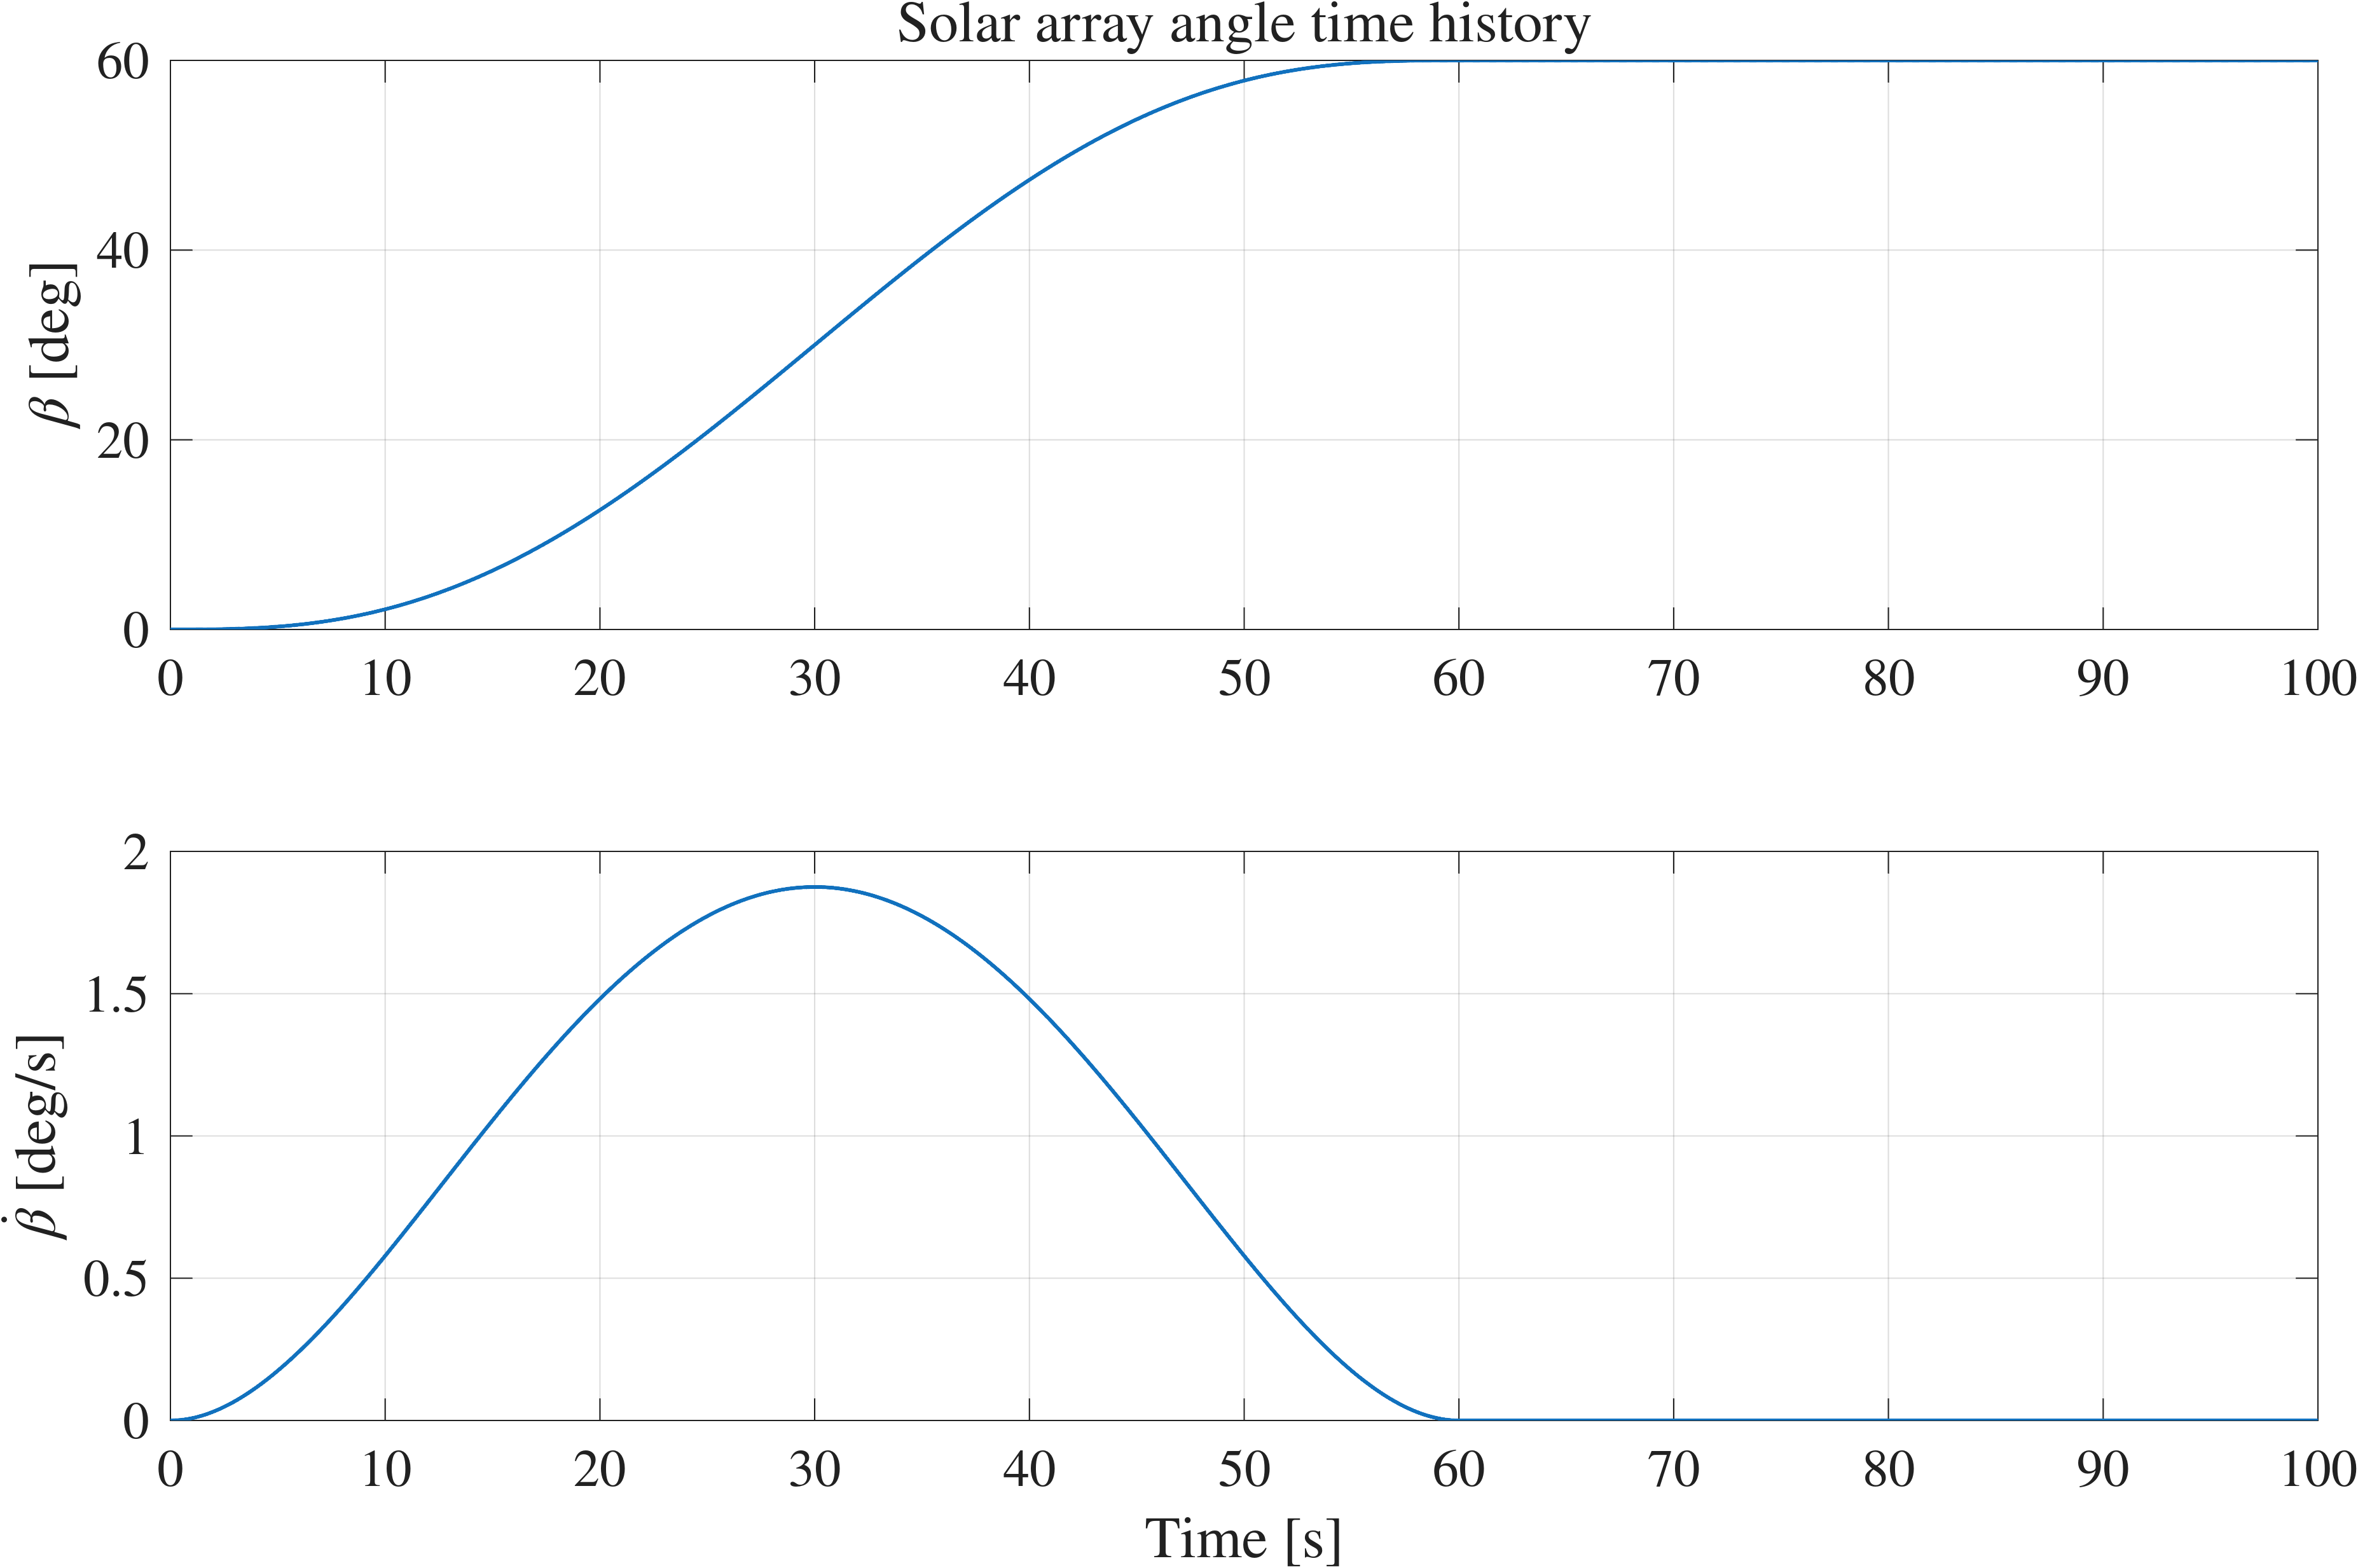
\includegraphics[width=0.8\textwidth]{b1_beta.png}
		\caption{Time histories of the array angle $\beta$ and rate $\dot{\beta}$ over $0\leq t\leq 100$}
		\label{fig:b1beta}
	\end{figure}
\end{mdframed}

\subsubsection*{(b.2): Find}

Implement the EoM derived above, and report the implemented code. Numerically propagate the system for $0\leq t\leq 100$ sec with $\boldsymbol{u}=\boldsymbol{0}$. Plot the time histories $\boldsymbol{\theta}$, $\boldsymbol{\omega}$, and $\boldsymbol{\Omega}$.\\

\textbf{Analysis/Conclusions:}\\

\end{document}